\documentclass{article}
\usepackage[utf8x]{inputenc}
\usepackage{graphicx}
\usepackage{amsmath}
\usepackage{amssymb}
\usepackage{tikz}
\usepackage{todonotes}
\usepackage{pgfplots}
\usepackage{epstopdf}
\usepackage{listings}
\usepackage{circuitikz}
\usepackage{float}
\usepackage{cleveref}
\usepackage{ragged2e} % For text alignment


\newenvironment{custom_itemize}{
\begin{itemize}
  \setlength{\itemsep}{0pt}
  \setlength{\parskip}{0pt}
  \setlength{\parsep}{0pt}
}{\end{itemize}}


\usepackage[hmarginratio=1:1,top=22mm,columnsep=16pt]{geometry} % Document margins
%\usepackage{multicol} % Used for the two-column layout of the document


%\usepackage{bm}


\title{NASA project}
\author{Kees Kroep 4246373}


\begin{document}
%  \twocolumn[{%
% \begin{@twocolumnfalse}
  \maketitle
%   \end{@twocolumnfalse}
% }]


\section*{Abstract}
Type an abstract

\clearpage
\tableofcontents
\clearpage

\section*{Introduction}
This document is a feasability study of a lidar sensor designed for the Europa Clipper. The main focus of this document will lie on the three most challenging aspects of the sensor design. How to achieve the target precision goals of the two modus of operation within the power budget, and the effect of radiation on the system.

First the requirements will be stated in \cref{ssec:high_level_specifications}, next the assumptions used for this study will be listed in ??,  then the feasability of the Altimetry Mode and Hazard Detection Mode will be investigated in ?? and ?? respectively. Section ?? will zoom into the effect of radiation on the system, and finally ?? and ?? will conclude the system with a spec sheet etc\dots

\section{Requirements and Specifications}\label{sec:requirements_and_specifications}
\section{High level specifications} 
\label{sec:high_level_specifications}
The radiation and mass, power and volume budget are listed in \cref{tab:req_radiation} and \cref{tab:req_mpv}.

\begin{table}[H]
\centering
\caption{Overview of radiation limitations}
\label{tab:req_radiation}
\begin{tabular}{|l|l|}
\hline
\textbf{Radiation}      &          \\ \hline
\begin{tabular}[c]{@{}l@{}}Total Integrated Dose in Silicon\\     behind 100 mil Al spherical shell\end{tabular} & 500 krad \\ \hline
\end{tabular}
\end{table}

\begin{table}[H]
\centering
\caption{Requirements for mass, power and volume}
\label{tab:req_mpv}
\begin{tabular}{|l|l|} \hline
\textbf{Mass, Power \& Volume Budget}                                 &               \\ \hline
Optical Head                                                 & \textless5 kg \\
Inside vault                                                 & \textless1 kg \\
\begin{tabular}[c]{@{}l@{}}Max cable length between \\ 
optical head and electronics\end{tabular} & 2 m           \\
Power                                                        & \textless50 W \\ \hline
\end{tabular}
\end{table}

The Lidar sensor features two operation modes: the Altimetry Mode, and the Hazard Detection Mode. 

\subsection{Altimetry Mode} 
\label{ssec:altimetry_mode}

Altimetry Mode is the first phase of the landing. During the Altimetry Mode, the Lidar sensor has to provide the altitude of the sensor in relationship to the surface op Europa. The requirements for the Altimetry Mode are listed in \cref{tab:req_altimetry}

\begin{table}[H]
\centering
\caption{Requirements for Altimetry Mode}
\label{tab:req_altimetry}
\begin{tabular}{|l|ll|} \hline
\textbf{Altimetry Mode}     & Threshold & Goal   \\ \hline
Max acquisition Slant Range & 5 km      & 8 km   \\
Range Accuracy (3-sigma)    & 1\%       & 0.10\% \\
Update Rate                 & 0.1 Hz    & 1 Hz   \\ \hline
\end{tabular}
\end{table}

\subsection{Hazard Detection Mode} 
\label{ssec:hazard_detection_mode}

During the Hazard Detection Mode a 3d map of the surface of Europa must be created around the landing place. The Hazard Mode is operational when the sensor is close enough to the surface of Europa. The requirements for the Hazard Detection Mode can be found in \cref{tab:req_hazard_detection}

\begin{table}[H]
\centering
\caption{Requirements for Hazard Detection Mode}
\label{tab:req_hazard_detection}
\begin{tabular}{|l|ll|} \hline
\textbf{Hazard Detection Mode}               & Threshold     & Goal          \\ \hline
Max range (altitude)                         & 400 m         & 500 m         \\
Min Operational Range (altitude)             & 5 m           & 1 m           \\
Range Accurcay (3-sigma on final 3D map)     & 10 cm         & 5 cm          \\
Ground Sample Distance (per pixel on 3D map) & 10 cm         & 5 cm          \\
Ground Area Coverage at max altitude         & 100 m x 100 m & 125 m x 125 m \\
Time for 3D map creation                     & 1 s           & 1 s           \\ \hline
\end{tabular}
\end{table}

%\section{System engineering level design} 
\label{sec:system_engineering_level_design}
In this section a system engineering level design is constructed that meets the performance requirements stated in \cref{sec:high_level_specifications}. \Cref{ssec:overview} shall provide an overview of the system, \cref{ssec:assumptions} shall list the assumptions made, and \cref{ssec:trade_offs_and_methodology} shall elaborate on trade-offs and design decisions. 

\section{Overview} 
\label{ssec:overview}
A schematic overview of the sensor is shown in \cref{tkz:schematic_overview}.

\begin{figure}[H]
    \centering



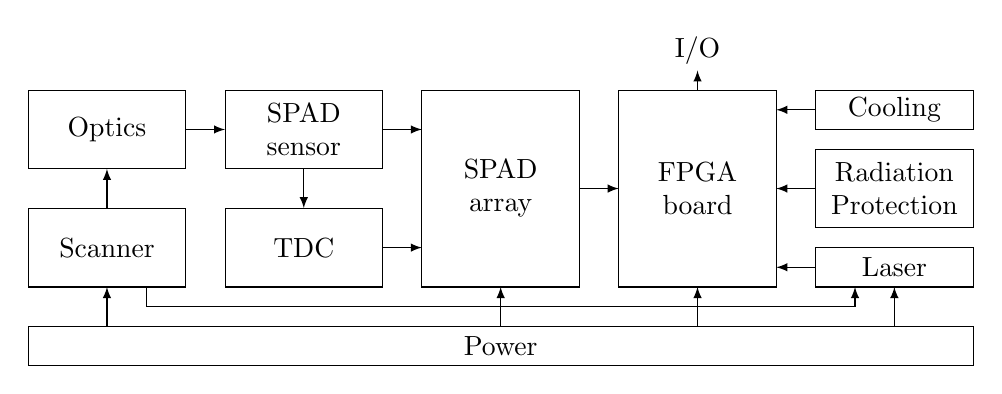
\begin{tikzpicture}[scale=.5]

\draw  (13,2) rectangle (17,1) node[pos=.5, align=center]{Cooling};
\draw  (13,0.5) rectangle (17,-1.5) node[pos=.5, align=center]{Radiation\\Protection};
\draw  (-7,-4) rectangle (17,-5) node[pos=.5, align=center]{Power};
\draw  (13,-2) rectangle (17,-3) node[pos=.5, align=center]{Laser};
\draw  (8,2) rectangle (12,-3) node[pos=.5, align=center]{FPGA\\board};
\draw  (3,2) rectangle (7,-3) node[pos=.5, align=center]{SPAD\\array};
\draw  (-2,2) rectangle (2,0) node[pos=.5, align=center]{SPAD\\sensor};
\draw  (-7,2) rectangle (-3,0) node[pos=.5, align=center]{Optics};
\draw  (-7,-1) rectangle (-3,-3) node[pos=.5, align=center]{Scanner};
\draw  (-2,-1) rectangle (2,-3) node[pos=.5, align=center]{TDC};

\draw [>=latex, ->](0,0) -- (0,-1);
\draw [>=latex, ->](2,-2) -- (3,-2);
\draw [>=latex, ->](13,1.5) -- (12,1.5);
\draw [>=latex, ->](7,-.5) -- (8,-.5);
\draw [>=latex, ->](2,1) -- (3,1);
\draw [>=latex, ->](13,-2.5) -- (12,-2.5);
\draw [>=latex, ->](10,2) -- (10,2.5);
\draw [>=latex, ->](-3,1) -- (-2,1);
\draw [>=latex, ->](13,-.5) -- (12,-.5);
\draw [>=latex, ->](5,-4) -- (5,-3);
\draw [>=latex, ->](10,-4) -- (10,-3);
\draw [>=latex, ->](15,-4) -- (15,-3);
\draw [>=latex, ->](-5,-1) -- (-5,0);
\node at (10,3) {I/O};

\draw [>=latex, ->](-5,-4) -- (-5,-3);
\draw [>=latex, ->](-4,-3) -- (-4,-3.5) -- (14,-3.5) -- (14,-3);

\end{tikzpicture}




    \caption{Schematic overview}
    \label{tkz:schematic_overview}
\end{figure}

~\\
\textbf{Laser}: The laser must send short pulses but powerful pulses at a predefined frequency, to transmit photons that can be detected by the SPAD Sensor. A critical requirement for the laser is the amount of photons it is able to transmit as a function of time, within the budget and technical limitations. \\
\\
\textbf{SPAD Sensor}: The Single Photon Avalanche Diode (SPAD) is responsible for generating a digital pulse when hit by a photon. A circuit build around the SPAD must ensure that the SPAD is quenched as quickly as possible to minimize the deadline. A critical requirement for the SPAD is a small jitter to maximize the accuracy of the sensor.  \\
\\
\textbf{TDC}: The Time Interval to Digital Converter (TDC) is connected to the laser and the SPAD Sensor. The TDC must measure the time difference between the transmission of the laser and the receiving at the SPAD sensor. This measurement requires an accuracy of tens of picoseconds to meet the accuracy requirements.\\
\\
\textbf{Scanner}: The scanner handles the scanning motion that is needed to accumulate the entire picture. Different scanning motions can introduce undesired jitter and heavily influence the amount of SPAD Sensors that are needed on teh SPAD Array. \\
\\
\textbf{SPAD Array}: The SPAD Array integrates the SPAD Sensors on a chip and connects them to the TDCs. The layout of the SPAD Array is closely related to the scanning motion that is used in the scanner.\\
\\
\textbf{Optics}:
The optics must transfer as much of the incoming photons as possible to the sensitive area on the SPAD Sensors. The Optics part also implements a bandpass filter around the target frequency. \\
\\
\textbf{FPGA Board}:
The FPGA Board controls the sensor. It is responsible for accumulating and interpreting the measurements from the TDCs, and controlling the Scanner and Laser. \\
\\
\textbf{Cooling}:
The cooling has to keep the temperature of the FPGA chip under a threshold temperature.\\
\\
\textbf{Radiation Protection}:
The Radiation Protection shields sensitive parts of the sensor from radiation. The most sensitive part of the system is expected to be the FPGA Board, based on experience.\\
\\
\textbf{Power}:
The power block has to supply the scanner, SPAD Array, FPGA Board, and the laser with the required power. The power block has to operate within the specified power budget.












\clearpage
\section{Assumptions} 
\label{ssec:assumptions}
This section will list the assumption that are made throughout the study.\\
\\
\textbf{Reflectivity of surface Europa}: It is assumed that out of all light that hit's Europa, $35\%$ is reflected in a perfectly diffuse manner.\\ 
\\
\textbf{Wavelength laser}: The wavelength of light emitted by the laser is assumed to be $850\,nm$. This wavelength is a typcial choice for Silicon SPAD's. The main reason for this wavelength as opposed to $550\,nm$ is because the that sunlight is less strong in that region, and less background noise will lft after applying a narrow bandpass filter. \\
\\
\textbf{Bandpass filter}:A bandpass filter will be used o filter background noise. This filter is assumed to be a bandpass filter with a center frequency of $850\,nm$ and a FWHM of $10\,nm$.The minimum transmission of the filter is $50\%$. These values are directly taken from the "\textit{850nm, 10nm FWHM, 12.5mm Mounted Diameter}" product made by Edmund Optics and sold for $75\,\$$.\\
\\
\textbf{Jitter of SPAD Sensor}: The jitter of the SPAD Sensor, or Full Width Half Max (FWHM) is assumed to be $100\,ps$. This value is a typical FWHM for state of the art Silicon SPAD's. \\
\\
\textbf{Jitter of TDC}: The jitter of the TDC's is assumed to be insignificant when compared to the jitter of $100\,ps$ caused by the SPAD Sensors. Experience with previous designs show that TDC jitter is generally a very small contributor to overall jitter.\\
\\
\textbf{Resolution of TDC}: The accuracy of the TDC is assumed to be $50\,ps$.\\
\\
\textbf{Sunlight}: It is assumed that the light from the sun that is reflected of Europa is the only signifant contributor to background noise. No other sources of light will be considered. \\
\\
\textbf{Photon Detection Probability}: It is assumed that the PDP of the SPADs is $10\%$.\\
\\
\textbf{Laser light hitting target}: It is assumed that all the light that leaves the laser is hitting the target area on Europa.
\\
\\
\textbf{Laser efficiency}: It is assumed that the laser has an efficiency of $10\%$.


\clearpage
\subsection{Trade-offs and Methodology} 
\label{ssec:trade_offs_and_methodology}
This section will list the trade-offs that can be found in the system. Each trade-off will be analyzed, and based on that, a decision will be made.


\subsubsection{High Frequency vs Low Frequency pulses}\label{sssec:high_low_freq}
The pulse frequency is limited by the roundtrip time  of the transmitted photons. The roundtrip time can be calculated using \cref{eq:roundtrip}

\begin{align}\label{eq:roundtrip}
t_{round} = \frac{2r}{c}
\end{align}
where $c\approx 3\cdot10^8$ is the speed of light, and $r$ the altitude of the sensor. The maximum pulse frequency can then be calculated using \cref{eq:pulse_f}

\begin{align}\label{eq:pulse_f}
f_{pulse} = \frac{1}{t_{round}} = \frac{c}{2r}
\end{align}

The maximum altitude are different for the Altimetry and Hazard Detection mode. The maximum pulse frequency of both modes is shown in \cref{tab:pulse_frequency}.

\input{tab/pulse_frequency_tab}

In order to increase the frequency, it is intersting to see what happens if the frequency is increased. The TDC measures the time between the last outgoing pulse and the incomming pulse. This means that the performed measurement $t_{TDC}$ can be calculated using \cref{eq:t_TDC_ToF}.

\begin{align}\label{eq:t_TDC_ToF}
	t_{TDC} &=ToF \mod T_{pulse}\\	
	ToF &= t_{TDC}+k\cdot T_{pulse} & k \in \mathbb{N}\label{eq:ToF_t_TDC}
\end{align}

 where $t_{TDC}$ is the measurement of the TDC, $ToF$ the time of flight, and $T_{pulse}$ the time period of the laser pulses. The returned answer is related to $ToF$ as shown in \cref{eq:ToF_t_TDC}. The precision of the measurement is maintained,  but on a larger scale the information is lost. \\
 \\
To solve this problem one can make measurements in two different frequencies. The idea is also applied in TDCs (Name of technique?), where two ring oscillators with different frequencies are used to amplify the range of the TDC. A similar idea can be applied here, but instead of using two oscillators, the time is devided in half, and in the first half the laser sends pulses in frequency $f_1$, and in the second half pulses with frequncy $f_2$. These two different measurements can first be used to determine the large scale ToF, and then the measurements can be combined to get a high accuracy to accompany that.\\
\\
As a proof of concept. This idea is applied to the Altimetry Mode. It is assumed that a difference of $5\,ns$ between $\lambda_1$ and $\lambda_2$ is sufficient. Now using a maximum $ToF$ one can calculate that optimal two frequencies, such that $f1_>f_2$ and $f_2$ as high as possible. 

\begin{align}
 	\frac{50\mu}{5n} &= 10660\\ 
 	\sqrt{\frac{50\mu}{5n}} &\approx 103
 \end{align} 
 Now two coprime numbers in $\mathbb{N}$ around 103 are 103 and 104. The resulting frequencies are
 \begin{align}
 	T_1 &= 103\cdot5n = 515n\\
 	T_2 &= 104\cdot5n = 520n\\
 	f_1 &= \frac{1}{T_1} = 1.9417\,MHz\\
 	f_2 &= \frac{1}{T_1} = 1.9231\,MHz\\
 \end{align}
The pulse frequency increases by a factor 100. A matlab plot of the resulting system is shown in \cref{fig:frequency_hopping}, where the measurement values of the TDC are plotted against the $ToF$.


\begin{figure}[h]
    \centering
    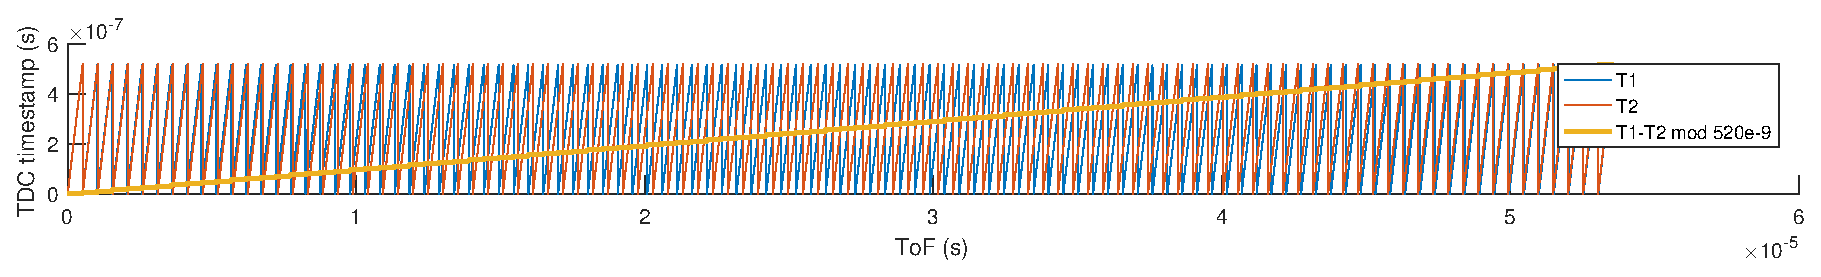
\includegraphics[width=\textwidth]{fig/frequency_hopping.eps}
    \caption{Matlab plot of TDC measurements vs ToF}
    \label{fig:frequency_hopping}
\end{figure}

The $ToF$ can be calculated using \cref{eq:ToF}.

\begin{align}
	t_{1-2} &= (t_1-t_2)\mod T_2\\
	ToF &= \frac{t_{1-2}}{T_2-T_1}T_1+\frac{t_1+t_2-t_{1-2}}{2}\label{eq:ToF}
\end{align}
where $t_1$ and $t_2$ are the timestamp measurements for $f_1$ and $f_2$ respectively. $t_{1-2}$ is the modulus of the time difference between $t_1$ and $t_2$.

\section{Optics}\label{ssec:optics}
The receiver optics are a good place to start of with, because the optics are not very dependent on results achieved in other areas. The optics have to transport as many desired photons, and as little unwanted photons to the active area on the SPADs as possible. All while having an acceptable depth of field. 

The most basic solution is a single lens with an aperture. The opacity of the lens can be calculated with the absorption of the lens material and f-number of the lens using \cref{eq:basic_opacity}.

\begin{align}\label{eq:basic_opacity}
\text{opacity} = \frac{1-\text{absorption}}{\text{f-number}^2}
\end{align}

 The performance of a possible configuration is shown in \cref{tab:basic_optics}

\input{tab/basic_optics_tab}

\subsection{Improvements}
There are a couple of additions that can improve the performance of the optics. The first and essential one, is the use of a bandpass filter. The transmitted signal will have a very specific bandwidth of $850\,nm$. Using a narrow bandpass filter one can filter out an enormous part of the background noise. The filter will have an opacity of $50\,\%$ for the target wavelength.

The captured photons that hit the lens need to be guided to the active area of the SPADs. If the active area on the chip is very small, one can use microlenses to improve the effectiveness of the optics. A Microlens focuses light on a single SPAD on the chip. Two types of microlenses will be considered: a spherical lens, and a square shaped lens. The presence of microlenses poses a limitation of the main lens. The f-number must be relatively large. A higher f-number means a smaller aperture and therefore more loss of photons. A way of dealing with this problem is to use a second lens instead. An overview of the available options is shown in \cref{tkz:receiver_optics}

\input{tkz/receiver_optics_tkz}

\begin{align}
\text{opacity} = (1-\text{absorption}_1)(1-\text{absorption}_2)\cdot\text{opacity filter}\cdot \frac{X}{\text{f-number}^2}
\end{align}
Where $X$ is the active area on the chip. A comparison between the different options is shown in \cref{tab:receiver_optics}

\input{tab/receiver_optics_tab}

The comparison in \cref{tab:receiver_optics} shows some good alternatives to the basic lens, if there is a need for it due to a small active area on the chip. However, most of the future calculations will focus on the basic model A.


\section{Scanning motion}\label{ssec:scanning_motion}
In \cref{ssec:SPADs}, it was concluded that a SPAD array with one SPAD per pixel is not feasible. Therefore a scanning motion is required. Possible scanning motions for different SPAD array configurations are shown in \cref{tkz:scanning_motions}. Note that the $2048\times1$ motion is in essence a special case of the $2048\times N$ motion, where exactly one row of pixels is observed at a time. The $M\times N$, with $M<2048$ and $N<2048$ needs a scanning motion in both $x$ and $y$ direction. This makes the scanning motion very complicated and unreliable. Therefore only the family of solutions with $2048\times N$ with $N<2048$ will be considered.


\input{tkz/scanning_motions_tkz}


\subsubsection{Background Noise}\label{ssec:background_noise}
For the background noise, it is assumed that the sun is the dominant source. The sum is modelled as an ideal black body. The spectral irradiance of the sun can be calculated using \cref{eq:spectral_irradiance}.
\begin{align}\label{eq:spectral_irradiance}
I_\lambda(\lambda,T) = \frac{2hc^2}{\lambda^5}\frac{1}{e^{\frac{hc}{\lambda kT}}-1}
\end{align}
where $I_\lambda(v,t)$ is spectral irradiance with unit $W/m^3$. \\
$h$ is the planck constant\\
$c$ is the speed of light in vacuum \\
$k$ is the Boltzman constant \\
$\lambda$ is the wavelength of the electromagnetic radiation\\
$T$ is the absolute temperature of the body\\
The spectral irradiance of the sun is calculated in \cref{tab:sun_irradiance}.

\input{tab/sun_irradiance_tab}

The next step is to calculate the power emitted by the sun in the specified bandwidth, at the location of Europa. This is done by modelling sun as a point source, and then spreading that power over a sphere with a radius equal to the distance between the sun and Europa, as is done in \cref{eq:point_source}.

\begin{align}\label{eq:point_source}
    P_{sun} = I_{\text{sun}} B_\lambda S \frac{r_{\text{sun}}^2}{r_{\text{europa}}^2}
\end{align}
where $I_{\text{sun}}$ is the spectral irradiance of the sun at the center frequency of the filter, $B_\lambda$ is the bandwidth of the filter in meters, $S$ the surface area of the target area on Europa, $r_{\text{sun}}$ the of radius of the sun, and $r_{\text{europa}}$ the distance between Europa and the sun. The effective radiance of the background noise at Europa is calculated in \cref{tab:power_background} using \cref{eq:point_source}.

\input{tab/effective_irradiance_tab}
\subsection{Resolution} 
\label{ssec:resolution}
The requirement for the altimetry mode changes based on the height. The target is a resolution of at least $0.1\,\%$. To ensure that this requirement is met, both the largest altitude of $8\,km$, and the smallest altitude of $500\,m$ will be investigated.

The minimum resolution for the largest and shortest altitude are $8\,m$ and $0.5\,m$ respectively. The maximum allowable FWHM can be calculated using \cref{eq:max_FWHM}.
 Using \cref{eq:FWHM_sigma} the maximum standard deviation can be calculated. The calculations are performed

\begin{align}\label{eq:max_FWHM}
FWHM_{max} = \frac{2x}{c}
\end{align}

\input{tab/AM_requirements_tab}







\subsubsection{standard deviation shortcut}
To calculate the standard deviation of the sum of multiple random variables that are independent and uncorrelated, one can use \cref{eq:variance_weighted_sum}


\begin{align}\label{eq:variance_weighted_sum}
\newcommand{\Var}{\mathrm{Var}}
 	\Var[aX+bY+cZ] = a^2\Var[X]+b^2\Var[Y]+c^2\Var[Z]
\end{align}




Next consider a situation where there are two random variable distributions. The first distribution is $S$, which is a normal distribution with $\mu_s=ToF$, where $ToF \in \{0, 50\mu\}$, and $\sigma_s=100p$. The second distribution is $N$, which is a uniform distribution with $\mu_n=\frac{50\mu}{2}$ and $\sigma_n=\frac{50\mu}{\sqrt{12}}$.

\begin{align}
	\mu_{mean} &= \frac{1}{110}\Big(\sum_{k=1}^{100}\mu_s+\sum_{l=1}^{10}\mu_n\Big)\\
			   &= \frac{100ToF+10*25\mu}{110}\\
			   &= \frac{10}{11}ToF+227.3n
\end{align}


\begin{align}
	\mathrm{Var}_{mean} &= \mathrm{Var}\Big[\frac{1}{110}\Big(\sum_{k=1}^{100}S_k+\sum_{l=1}^{10}N_l\Big)\Big]\\ 
	 &= \frac{1}{110^2}\Big(\sum_{k=1}^{100}\mathrm{Var}[S]+\sum_{l=1}^{10}\mathrm{Var}[N]\Big)\\
	&= \frac{1}{110^2}(100\sigma_s^2+10\sigma_n^2)\\
	&= \frac{10^{-18}+2.0833\cdot10^{-9}}{110^2}\\
	&= 1.7218\cdot10^{-13}\\
	\sigma_{mean} &= \sqrt{\mathrm{Var}_{mean}}\\
				  &= 414.94n
\end{align}



% Now we grab 100 samples out of $S$ and 10 out of $N$. First, the $\sigma$ and $\mu$ of the average of the 100 samples of $S$ is calculated.

% \begin{align}
% 	\mu_{s,mean} &= \frac{1}{100}\sum_{k=1}^{100}\mu_s\\
% 			     &= ToF
% \end{align}

% \begin{align}
% 	\mathrm{Var}[\frac{1}{100}\sum_{k=1}^{100}S_k] &= \frac{1}{100^2}\sum_{k=1}^{100} \mathrm{Var}[S_k]\\
% 						  &= \frac{\mathrm{Var}[S]}{100}\\
% 	\sigma_{s,mean} &= \frac{\sigma_s}{\sqrt{100}}\\
% 					&= 10p
% \end{align}

% Next the average of 10 samples of $N$ is calculated.

% \begin{align}
% 	\mu_{n,mean} &= \frac{1}{10}\sum_{k=1}^{10}\mu_n\\
% 			     &= 25\mu
% \end{align}

% \begin{align}
% 	\mathrm{Var}[\frac{1}{10}\sum_{k=1}^{10}] &= \frac{1}{10^2}\sum_{k=1}^{10} \mathrm{Var}[N_k]\\
% 						  &= \frac{\mathrm{Var}[N]}{10}\\
% 	\sigma_{s,mean} &= \frac{\sigma_n}{\sqrt{10}}\\
% 					&= \frac{50\mu}{\sqrt{120}}
% 					&\approx 4.5644\mu
% \end{align}

% Next the two resulting functions are combined






% \subsection{Laser}
The laser is responsible for the photons that are used for the Time of Flight (ToF) measurement. The laser has to ensure that the Signal to Background Noise Ratio (SBNR) is at least 0 dB. The power budget of the entire system is $50\,W$, which is the main bottleneck for the performance of the laser. The wavelength of the laser is $850\,nm$. The $P_B$ is already calculated in \cref{ssec:background_noise}. In order to achieve an SNR of 0 dB, the signal power $P_S$ must therefore at least match the background noise power that hits the surface of Europa. One can calculate the signal power at the optics using \cref{eq:P_S}.

\begin{align}\label{eq:P_S}
	P_S = P_{pulse} \cdot f_{pulse} \cdot R_{\text{Europa}}
\end{align}
where $P_{pulse}$ is the power of a single pulse of the laser, $f_{pulse}$ the frequency at which the pulses are transmitted, $R_{\text{Europa}}$ the reflectivity of Europa, and $r$ the altitude from the sensor to the surface of Europa. The SBNR can then be calculated using \cref{eq:SBNR}.

\begin{align}\label{eq:SBNR}
	SBNR &= \frac{P_S}{P_B}
\end{align}

The power of a single pulse can be calculated by combining \cref{eq:P_S} and \cref{eq:SBNR} into \cref{eq:p_pulse}. This is done in \cref{tab:p_pulse}.

\begin{align}
	P_{pulse} &= \frac{P_B\cdot SBNR}{f_{pulse}\cdot R_{\text{Europa}}}
\end{align}

\input{tab/p_pulse_tab}

The $P_{pulse}$ is the optical power that is emitted by the laser. The electrical power is $\frac{P_{pulse}}{0.1}=3.4\,W$, which is well within the power envelope of $50\,W$. The next step is to calculate the required peak power $p_{peak}$ of the laser, using \cref{eq:p_peak}

\begin{align}\label{eq:p_peak}
 	P_{peak} &= \frac{P_{pulse}}{t_{pulse} \cdot f_{pulse}}
 \end{align} 
where $P_{peak}$ is the peak power and $t_{pulse}$ the FWHM of a pulse.

Using a typical pulse width of $t_{pulse} = 100\,ns$ and the $f_{pulse}$ as calculated in \cref{ssec:high_low_freq} one gets the result shown in \cref{tab:p_peak}.

\input{tab/p_peak_tab}















\section{Overview} 
\label{ssec:overview}
A schematic overview of the sensor is shown in \cref{tkz:schematic_overview}.

\begin{figure}[H]
    \centering



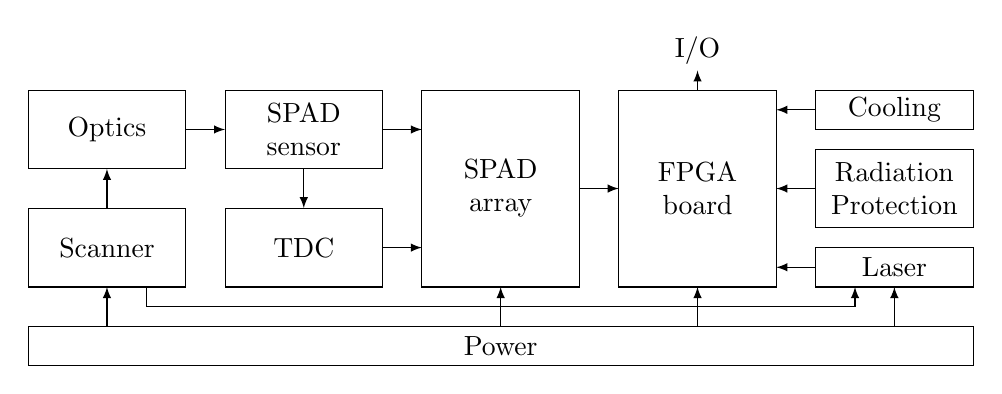
\begin{tikzpicture}[scale=.5]

\draw  (13,2) rectangle (17,1) node[pos=.5, align=center]{Cooling};
\draw  (13,0.5) rectangle (17,-1.5) node[pos=.5, align=center]{Radiation\\Protection};
\draw  (-7,-4) rectangle (17,-5) node[pos=.5, align=center]{Power};
\draw  (13,-2) rectangle (17,-3) node[pos=.5, align=center]{Laser};
\draw  (8,2) rectangle (12,-3) node[pos=.5, align=center]{FPGA\\board};
\draw  (3,2) rectangle (7,-3) node[pos=.5, align=center]{SPAD\\array};
\draw  (-2,2) rectangle (2,0) node[pos=.5, align=center]{SPAD\\sensor};
\draw  (-7,2) rectangle (-3,0) node[pos=.5, align=center]{Optics};
\draw  (-7,-1) rectangle (-3,-3) node[pos=.5, align=center]{Scanner};
\draw  (-2,-1) rectangle (2,-3) node[pos=.5, align=center]{TDC};

\draw [>=latex, ->](0,0) -- (0,-1);
\draw [>=latex, ->](2,-2) -- (3,-2);
\draw [>=latex, ->](13,1.5) -- (12,1.5);
\draw [>=latex, ->](7,-.5) -- (8,-.5);
\draw [>=latex, ->](2,1) -- (3,1);
\draw [>=latex, ->](13,-2.5) -- (12,-2.5);
\draw [>=latex, ->](10,2) -- (10,2.5);
\draw [>=latex, ->](-3,1) -- (-2,1);
\draw [>=latex, ->](13,-.5) -- (12,-.5);
\draw [>=latex, ->](5,-4) -- (5,-3);
\draw [>=latex, ->](10,-4) -- (10,-3);
\draw [>=latex, ->](15,-4) -- (15,-3);
\draw [>=latex, ->](-5,-1) -- (-5,0);
\node at (10,3) {I/O};

\draw [>=latex, ->](-5,-4) -- (-5,-3);
\draw [>=latex, ->](-4,-3) -- (-4,-3.5) -- (14,-3.5) -- (14,-3);

\end{tikzpicture}




    \caption{Schematic overview}
    \label{tkz:schematic_overview}
\end{figure}

~\\
\textbf{Laser}: The laser must send short pulses but powerful pulses at a predefined frequency, to transmit photons that can be detected by the SPAD Sensor. A critical requirement for the laser is the amount of photons it is able to transmit as a function of time, within the budget and technical limitations. \\
\\
\textbf{SPAD Sensor}: The Single Photon Avalanche Diode (SPAD) is responsible for generating a digital pulse when hit by a photon. A circuit build around the SPAD must ensure that the SPAD is quenched as quickly as possible to minimize the deadline. A critical requirement for the SPAD is a small jitter to maximize the accuracy of the sensor.  \\
\\
\textbf{TDC}: The Time Interval to Digital Converter (TDC) is connected to the laser and the SPAD Sensor. The TDC must measure the time difference between the transmission of the laser and the receiving at the SPAD sensor. This measurement requires an accuracy of tens of picoseconds to meet the accuracy requirements.\\
\\
\textbf{Scanner}: The scanner handles the scanning motion that is needed to accumulate the entire picture. Different scanning motions can introduce undesired jitter and heavily influence the amount of SPAD Sensors that are needed on teh SPAD Array. \\
\\
\textbf{SPAD Array}: The SPAD Array integrates the SPAD Sensors on a chip and connects them to the TDCs. The layout of the SPAD Array is closely related to the scanning motion that is used in the scanner.\\
\\
\textbf{Optics}:
The optics must transfer as much of the incoming photons as possible to the sensitive area on the SPAD Sensors. The Optics part also implements a bandpass filter around the target frequency. \\
\\
\textbf{FPGA Board}:
The FPGA Board controls the sensor. It is responsible for accumulating and interpreting the measurements from the TDCs, and controlling the Scanner and Laser. \\
\\
\textbf{Cooling}:
The cooling has to keep the temperature of the FPGA chip under a threshold temperature.\\
\\
\textbf{Radiation Protection}:
The Radiation Protection shields sensitive parts of the sensor from radiation. The most sensitive part of the system is expected to be the FPGA Board, based on experience.\\
\\
\textbf{Power}:
The power block has to supply the scanner, SPAD Array, FPGA Board, and the laser with the required power. The power block has to operate within the specified power budget.











\section{Assumptions} 
\label{ssec:assumptions}
This section will list the assumption that are made throughout the study.\\
\\
\textbf{Reflectivity of surface Europa}: It is assumed that out of all light that hit's Europa, $35\%$ is reflected in a perfectly diffuse manner.\\ 
\\
\textbf{Wavelength laser}: The wavelength of light emitted by the laser is assumed to be $850\,nm$. This wavelength is a typcial choice for Silicon SPAD's. The main reason for this wavelength as opposed to $550\,nm$ is because the that sunlight is less strong in that region, and less background noise will lft after applying a narrow bandpass filter. \\
\\
\textbf{Bandpass filter}:A bandpass filter will be used o filter background noise. This filter is assumed to be a bandpass filter with a center frequency of $850\,nm$ and a FWHM of $10\,nm$.The minimum transmission of the filter is $50\%$. These values are directly taken from the "\textit{850nm, 10nm FWHM, 12.5mm Mounted Diameter}" product made by Edmund Optics and sold for $75\,\$$.\\
\\
\textbf{Jitter of SPAD Sensor}: The jitter of the SPAD Sensor, or Full Width Half Max (FWHM) is assumed to be $100\,ps$. This value is a typical FWHM for state of the art Silicon SPAD's. \\
\\
\textbf{Jitter of TDC}: The jitter of the TDC's is assumed to be insignificant when compared to the jitter of $100\,ps$ caused by the SPAD Sensors. Experience with previous designs show that TDC jitter is generally a very small contributor to overall jitter.\\
\\
\textbf{Resolution of TDC}: The accuracy of the TDC is assumed to be $50\,ps$.\\
\\
\textbf{Sunlight}: It is assumed that the light from the sun that is reflected of Europa is the only signifant contributor to background noise. No other sources of light will be considered. \\
\\
\textbf{Photon Detection Probability}: It is assumed that the PDP of the SPADs is $10\%$.\\
\\
\textbf{Laser light hitting target}: It is assumed that all the light that leaves the laser is hitting the target area on Europa.
\\
\\
\textbf{Laser efficiency}: It is assumed that the laser has an efficiency of $10\%$.


\section{Altimetry Mode}\label{sec:altimetry_mode}
The Altimetry Mode is the mode in which only the altitude of the device in relationship to Europa is required. The main challenges for the altimetry mode are acquiring the required resolution, acquiring the required speed, staying within the power budget, and being sufficiently resilient against the accumulated radiation for the entire trip.

The first step will be to create a model of the noise that will be present at Europa. Then the required amount of signal will be calculated, resulting in the required signal power. 

\section{Optics}\label{ssec:optics}
The receiver optics are a good place to start of with, because the optics are not very dependent on results achieved in other areas. The optics have to transport as many desired photons, and as little unwanted photons to the active area on the SPADs as possible. All while having an acceptable depth of field. 

The most basic solution is a single lens with an aperture. The opacity of the lens can be calculated with the absorption of the lens material and f-number of the lens using \cref{eq:basic_opacity}.

\begin{align}\label{eq:basic_opacity}
\text{opacity} = \frac{1-\text{absorption}}{\text{f-number}^2}
\end{align}

 The performance of a possible configuration is shown in \cref{tab:basic_optics}

\begin{table}[H]
\centering
\caption{Performance of basic optics solution}
\label{tab:basic_optics}
\begin{tabular}{|l|r|}\hline
    \textbf{Basic Optics} & \\
    \hline 
    f-number & $2.00\, $ \\
    absorption & $5.00\,\%$ \\
    opacity & $23.75\, \%$ \\
    \hline 
\end{tabular}
\end{table}


\subsection{Improvements}
There are a couple of additions that can improve the performance of the optics. The first and essential one, is the use of a bandpass filter. The transmitted signal will have a very specific bandwidth of $850\,nm$. Using a narrow bandpass filter one can filter out an enormous part of the background noise. The filter will have an opacity of $50\,\%$ for the target wavelength.

The captured photons that hit the lens need to be guided to the active area of the SPADs. If the active area on the chip is very small, one can use microlenses to improve the effectiveness of the optics. A Microlens focuses light on a single SPAD on the chip. Two types of microlenses will be considered: a spherical lens, and a square shaped lens. The presence of microlenses poses a limitation of the main lens. The f-number must be relatively large. A higher f-number means a smaller aperture and therefore more loss of photons. A way of dealing with this problem is to use a second lens instead. An overview of the available options is shown in \cref{tkz:receiver_optics}

\begin{figure}[H]
    \centering


\resizebox{\linewidth*3/4}{!}{
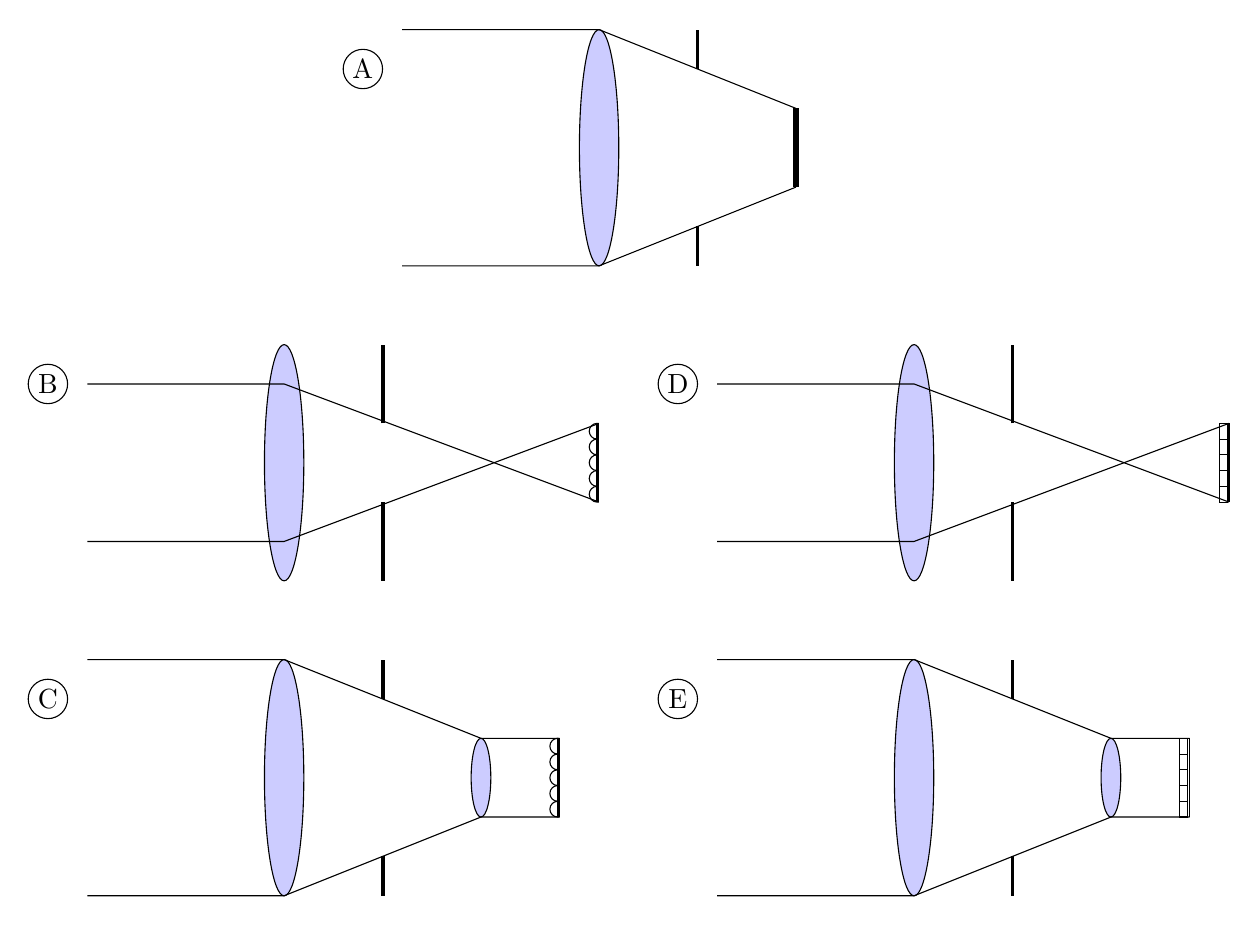
\begin{tikzpicture}[scale=.5]

%%%%%% low F-number, no microlens

%lens
\draw [fill=blue!20] (7,4) ellipse (0.5 and 3);

%diafragma
\draw [line width=.5mm] (9.5,6) -- (9.5,7);
\draw [line width=.5mm] (9.5,1) -- (9.5,2);

%sensitive area
\draw [line width=.7mm] (12,3) -- (12,5);

%light beams
\draw (2,7) to (7,7) to (12,5);
\draw (2,1) to (7,1) to (12,3);

%%%%%%Microlens + high F-number

%lens
\draw [fill=blue!20] (-1,-4) ellipse (0.5 and 3);

%diafragma
\draw [line width=.5mm] (1.5,-3) -- (1.5,-1);
\draw [line width=.5mm] (1.5,-7) -- (1.5,-5);

%sensitive area
\draw [line width=.7mm] (7,-5) -- (7,-3);

%light beams
\draw (-6,-2) to (-1,-2) to (7,-5);
\draw (-6,-6) to (-1,-6) to (7,-3) node (v1) {};


%Microlenses
\draw  (6.95,-3.2) ellipse (.2 and .2);
\draw  (6.95,-3.6) ellipse (.2 and .2);
\draw  (6.95,-4.0) ellipse (.2 and .2);
\draw  (6.95,-4.4) ellipse (.2 and .2);
\draw  (6.95,-4.8) ellipse (.2 and .2);
\fill  (7,-2.8) rectangle (7.4,-5.2) [fill=white];

%%%%%%Microlens + extra lens

%lens
\draw [fill=blue!20] (-1,-12) ellipse (0.5 and 3);

%second lens
\draw [fill=blue!20] (4,-12) ellipse (0.25 and 1);

%diafragma
\draw [line width=.5mm] (1.5,-10) -- (1.5,-9);
\draw [line width=.5mm] (1.5,-15) -- (1.5,-14);

%sensitive area
\draw [line width=.75mm] (6,-13) -- (6,-11);

%light beams
\draw (-6,-9) to (-1,-9) to (4,-11) to (6,-11);
\draw (-6,-15) to (-1,-15) to (4,-13) to (6,-13);


%Microlenses
\draw  (5.95,-11.2) ellipse (.2 and .2);
\draw  (5.95,-11.6) ellipse (.2 and .2);
\draw  (5.95,-12) ellipse (.2 and .2);
\draw  (5.95,-12.4) ellipse (.2 and .2);
\draw  (5.95,-12.8) ellipse (.2 and .2);
\fill  (6,-10.8) rectangle (6.4,-13.2) [fill=white];

%%%%%% Square Microlens + high F-number

%lens
\draw [fill=blue!20] (15,-4) ellipse (0.5 and 3);

%diafragma
\draw [line width=.5mm] (17.5,-3) -- (17.5,-1);
\draw [line width=.5mm] (17.5,-7) -- (17.5,-5);

%sensitive area
\draw  (23,-5) -- (23,-3);

%light beams
\draw (10,-2) to (15,-2) to (23,-5);
\draw (10,-6) to (15,-6) to (23,-3);


%Microlenses
\draw  (22.75,-3) rectangle (22.95,-3.4);
\draw  (22.75,-3.4) rectangle (22.95,-3.8);
\draw  (22.75,-3.8) rectangle (22.95,-4.2);
\draw  (22.75,-4.2) rectangle (22.95,-4.6);
\draw  (22.75,-4.6) rectangle (22.95,-5);


%%%%%% Square Microlens + extra lens

%lens
\draw [fill=blue!20] (15,-12) ellipse (0.5 and 3);

%second lens
\draw [fill=blue!20] (20,-12) ellipse (0.25 and 1);

%diafragma
\draw [line width=.5mm] (17.5,-10) -- (17.5,-9);
\draw [line width=.5mm] (17.5,-15) -- (17.5,-14);

%sensitive area
\draw  (22,-13) -- (22,-11);

%light beams
\draw (10,-9) to (15,-9) to (20,-11) to (22,-11);
\draw (10,-15) to (15,-15) to (20,-13) to (22,-13);


%Microlenses
\draw  (21.75,-11) rectangle (21.95,-11.4);
\draw  (21.75,-11.4) rectangle (21.95,-11.8);
\draw  (21.75,-11.8) rectangle (21.95,-12.2);
\draw  (21.75,-12.2) rectangle (21.95,-12.6);
\draw  (21.75,-12.6) rectangle (21.95,-13);



\draw  (1,6) ellipse (.5 and .5) node[]{A};
\draw  (-7,-2) ellipse (.5 and .5) node[]{B};
\draw  (-7,-10) ellipse (.5 and .5) node[]{C};
\draw  (9,-2) ellipse (.5 and .5) node[]{D};
\draw  (9,-10) ellipse (.5 and .5) node[]{E};


\end{tikzpicture}
}

    \caption{Overview of possible receiver optics implementations}
    \label{tkz:receiver_optics}
\end{figure}

\begin{align}
\text{opacity} = (1-\text{absorption}_1)(1-\text{absorption}_2)\cdot\text{opacity filter}\cdot \frac{X}{\text{f-number}^2}
\end{align}
Where $X$ is the active area on the chip. A comparison between the different options is shown in \cref{tab:receiver_optics}

\begin{table}[H]
\centering
\caption{comparison of different optics solutions}
\label{tab:receiver_optics}
\begin{tabular}{|l|lllll|}\hline
\textbf{Type}                & \textbf{A}        & \textbf{B}        & \textbf{C}        & \textbf{D}        & \textbf{E}        \\ \hline
absorption $1^{st}$ lens & 0.05     & 0.05     & 0.05     & 0.05     & 0.05     \\
f-number                 & 2        & 8        & 2        & 8        & 2        \\
absorption $2^{nd}$ lens & 0        & 0        & 0.05     & 0        & 0.05     \\
active area on chip      & 0.05     & 0.55     & 0.55     & 0.65     & 0.65     \\ \hline
effective opacity            & 0.011875 & 0.008164 & 0.124094 & 0.009648 & 0.146656 \\ \hline
\end{tabular}
\end{table}

The comparison in \cref{tab:receiver_optics} shows some good alternatives to the basic lens, if there is a need for it due to a small active area on the chip. However, most of the future calculations will focus on the basic model A.


\section{Noise caused by the sun}\label{ssec:background_noise}
The sun is the most dominant source of unwanted photons at Europa. This section will investigate how much energy is hitting the surface of Europa. 

To calculate that the sun will be modelled as an ideal black body. The spectral irradiance of the sun can be calculated using \cref{eq:spectral_irradiance}.
\begin{align}\label{eq:spectral_irradiance}
I_\lambda(\lambda,T) = \frac{2hc^2}{\lambda^5}\frac{1}{e^{\frac{hc}{\lambda kT}}-1}
\end{align}
where $I_\lambda(v,t)$ is spectral irradiance with unit $W/m^3$. \\
$h$ is the planck constant\\
$c$ is the speed of light in vacuum \\
$k$ is the Boltzman constant \\
$\lambda$ is the wavelength of the electromagnetic radiation\\
$T$ is the absolute temperature of the body\\



The spectral irradiance of the sun is calculated in \cref{tab:sun_irradiation}.

\begin{table}[H]
\centering
\caption{Calculation of sun irradiation}
\label{tab:sun_irradiation}
\begin{tabular}{|l|l|}\hline
    \textbf{Sun irradiation} & \\
    \hline 
    $h$ & $663.00\cdot10^{-36}\,Js$ \\
    $c$ & $300.00\cdot10^6\,m/s$ \\
    $k$ & $13.80\cdot10^{-24}\,j/K$ \\
    $\lambda$ & $850.00\,n m$ \\
    $I_\lambda$ & $15.11\cdot10^{12}\,W/m^3$ \\
    \hline 
\end{tabular}
\end{table}


The next step is to calculate the power emitted by the sun in the specified bandwidth, at the location of Europa. The specified bandwidth is in this case the assumed bandpass filter used on the lens. The emitted power is calculated by modelling the sun as a point source, and then spreading that power over a sphere with a radius equal to the distance between the sun and Europa, as is done in \cref{eq:point_source}.

\begin{align}\label{eq:point_source}
    P_{sun} = I_{\text{sun}} B_\lambda S \frac{r_{\text{sun}}^2}{r_{\text{europa}}^2}
\end{align}
where $I_{\text{sun}}$ is the spectral irradiance of the sun at the center frequency of the filter, $B_\lambda$ is the bandwidth of the filter in meters, $S$ the surface area of the target area on Europa, $r_{\text{sun}}$ the of radius of the sun, and $r_{\text{europa}}$ the distance between Europa and the sun. The effective radiance of the background noise at Europa is calculated in \cref{tab:background_power} using \cref{eq:point_source}.

\begin{table}[H]
\centering
\caption{Calculation of background power on target area on Europa}
\label{tab:background_power}
\begin{tabular}{|l|r|}\hline
    \textbf{Background power} & \\
    \hline 
    $I_\lambda$ & $15.11\cdot10^{12}\,W/M^3$ \\
    $B_\lambda$ & $10.00\,n m$ \\
    Surface area & $10000.00\, m^2$ \\
    $r_{sun}$ & $695.70\,\,km$ \\
    $r_{europa}$ & $800.00\cdot10^3\,km$ \\
    $P_B$ & $1.14\,k W$ \\
    \hline 
\end{tabular}
\end{table}


The next step is to calculate the percentage of energy that hits the device when hovering over Europa. The focal length and aperture ofthe lens will be configured in such a way that the target surface on Europa fills the entire view at the maximum altitude of the Hazard Detection Mode, so that altitude will be chosen to calculate the received noise power. The amount of power received at the lens of the device can be calculated using \cref{eq:power_lens}.

\begin{align}\label{eq:power_lens}
P'_B = \frac{P_B\cdot R_{Europa}\cdot D_l\cdot \text{opacity}}{2r^2}
\end{align}
where $P'_B$ is the power hitting the lens, \\
$P_B$ the noise power on the target area of Europa,\\
$R_{Europa}$ the reflectivity of Europa,\\
$D_l$ the diameter of the lens,\\
opacity the opacity of the lens,\\
and $r$ the altitude of the device. The calculations are performed in \cref{tab:effective_noise_power}.

\begin{table}[H]
\centering
\caption{Pulse frequency for both modes of operation}
\label{tab:effective_noise_power}
\begin{tabular}{|l|r|}\hline
    \textbf{effective noise power} & \\
    \hline 
    $P_B$ & $1.89\,m W$ \\
    $r$ & $500.00\, m$ \\
    $R_{europa}$ & $35.00\, \%$ \\
    Diameter lens $(D_l)$ & $50.00\,m m$ \\
    opacity filter $(L_f)$ & $50.00\, \%$ \\
    opacity optics $(L_l)$ & $14.60\, \%$ \\
    $P_B2$ & $4.82\,p W$ \\
    \hline 
\end{tabular}
\end{table}


Finally the power needs to be converted to number of photons. To calculate how many photons bounce from the surface of Europa and actually hit the light. To calculate the amount of photons one needs to know the amount of energy per photon. This can be calculated using \cref{eq:e_photon}. The calculation is performed in \cref{tab:energy_of_photon}.

\begin{align}\label{eq:e_photon}
E_{photon} = \frac{hc}{\lambda}
\end{align}

\begin{table}[H]
\centering
\caption{Pulse frequency for both modes of operation}
\label{tab:energy_of_photon}
\begin{tabular}{|l|r|}\hline
    \textbf{energy of photon} & \\
    \hline 
    $h$ & $663.00\cdot10^{-36}\,Js$ \\
    $c$ & $300.00\cdot10^6\,m/s$ \\
    $\lambda$ & $850.00\,n m$ \\
    $E_{photon}$ & $234.00\cdot10^{-21}\,J$ \\
    \hline 
\end{tabular}
\end{table}
 

The amout of photons per second can then be calculated using \cref{eq:PPS}. The calculation is shown in

\begin{align}\label{eq:PPS}
\text{photon}/s = \frac{P}{E_{photon}}
\end{align}

\begin{table}[H]
\centering
\caption{Pulse frequency for both modes of operation}
\label{tab:photons_hitting_SPADs}
\begin{tabular}{|l|r|}\hline
    \textbf{photons hitting SPADs} & \\
    \hline 
    $P'_B$ & $7.76\cdot10^{-6}\,W$ \\
    $E_{photon}$ & $2.34\cdot10^{-19}\,J$ \\
    photons at SPADs & $3.31\cdot10^{13}\,\text{photon}/s$ \\
    \hline 
\end{tabular}
\end{table}













% \subsubsection{High Frequency vs Low Frequency pulses}\label{sssec:high_low_freq}
The pulse frequency is limited by the roundtrip time  of the transmitted photons. The roundtrip time can be calculated using \cref{eq:roundtrip}

\begin{align}\label{eq:roundtrip}
t_{round} = \frac{2r}{c}
\end{align}
where $c\approx 3\cdot10^8$ is the speed of light, and $r$ the altitude of the sensor. The maximum pulse frequency can then be calculated using \cref{eq:pulse_f}

\begin{align}\label{eq:pulse_f}
f_{pulse} = \frac{1}{t_{round}} = \frac{c}{2r}
\end{align}

The maximum altitude are different for the Altimetry and Hazard Detection mode. The maximum pulse frequency of both modes is shown in \cref{tab:pulse_frequency}.

\begin{table}[H]
\centering
\caption{Pulse frequency for both modes}
\label{tab:pulse_frequency}
\begin{tabular}{|l|ll|}
\hline
\textbf{Pulse Frequency}      &      Altimetry & Hazard Detection    \\ \hline
Maximum altitude  &  $8\,km$ & $500\, m$\\ 
Roundtrip time      &  $53.3\,\mu s$ & $3.33\,\mu s$ \\
Pulse frequency     & $18.75\,kHz$    & $300\,kHz$  \\ \hline
\end{tabular}
\end{table}


In order to increase the frequency, it is intersting to see what happens if the frequency is increased. The TDC measures the time between the last outgoing pulse and the incomming pulse. This means that the performed measurement $t_{TDC}$ can be calculated using \cref{eq:t_TDC_ToF}.

\begin{align}\label{eq:t_TDC_ToF}
	t_{TDC} &=ToF \mod T_{pulse}\\	
	ToF &= t_{TDC}+k\cdot T_{pulse} & k \in \mathbb{N}\label{eq:ToF_t_TDC}
\end{align}

 where $t_{TDC}$ is the measurement of the TDC, $ToF$ the time of flight, and $T_{pulse}$ the time period of the laser pulses. The returned answer is related to $ToF$ as shown in \cref{eq:ToF_t_TDC}. The precision of the measurement is maintained,  but on a larger scale the information is lost. \\
 \\
To solve this problem one can make measurements in two different frequencies. The idea is also applied in TDCs (Name of technique?), where two ring oscillators with different frequencies are used to amplify the range of the TDC. A similar idea can be applied here, but instead of using two oscillators, the time is devided in half, and in the first half the laser sends pulses in frequency $f_1$, and in the second half pulses with frequncy $f_2$. These two different measurements can first be used to determine the large scale ToF, and then the measurements can be combined to get a high accuracy to accompany that.\\
\\
As a proof of concept. This idea is applied to the Altimetry Mode. It is assumed that a difference of $5\,ns$ between $\lambda_1$ and $\lambda_2$ is sufficient. Now using a maximum $ToF$ one can calculate that optimal two frequencies, such that $f1_>f_2$ and $f_2$ as high as possible. 

\begin{align}
 	\frac{50\mu}{5n} &= 10660\\ 
 	\sqrt{\frac{50\mu}{5n}} &\approx 103
 \end{align} 
 Now two coprime numbers in $\mathbb{N}$ around 103 are 103 and 104. The resulting frequencies are
 \begin{align}
 	T_1 &= 103\cdot5n = 515n\\
 	T_2 &= 104\cdot5n = 520n\\
 	f_1 &= \frac{1}{T_1} = 1.9417\,MHz\\
 	f_2 &= \frac{1}{T_1} = 1.9231\,MHz\\
 \end{align}
The pulse frequency increases by a factor 100. A matlab plot of the resulting system is shown in \cref{fig:frequency_hopping}, where the measurement values of the TDC are plotted against the $ToF$.


\begin{figure}[h]
    \centering
    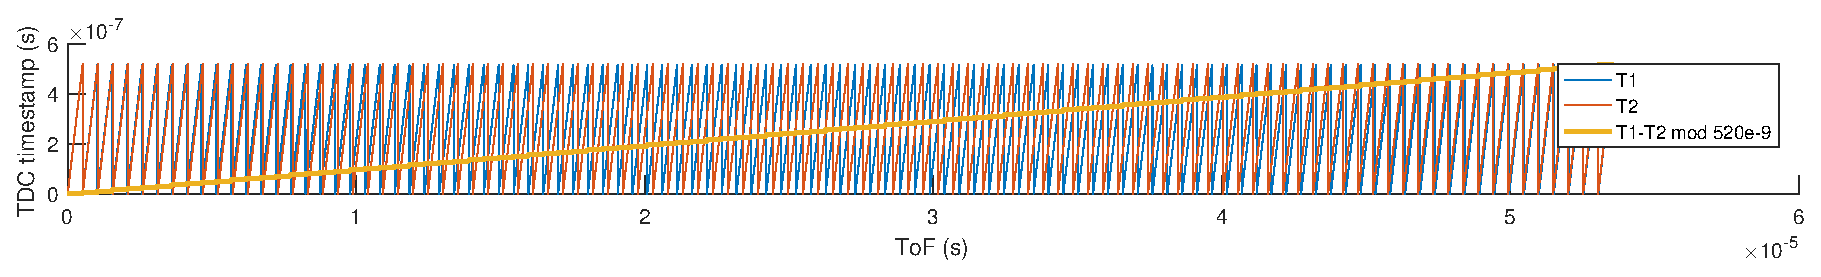
\includegraphics[width=\textwidth]{fig/frequency_hopping.eps}
    \caption{Matlab plot of TDC measurements vs ToF}
    \label{fig:frequency_hopping}
\end{figure}

The $ToF$ can be calculated using \cref{eq:ToF}.

\begin{align}
	t_{1-2} &= (t_1-t_2)\mod T_2\\
	ToF &= \frac{t_{1-2}}{T_2-T_1}T_1+\frac{t_1+t_2-t_{1-2}}{2}\label{eq:ToF}
\end{align}
where $t_1$ and $t_2$ are the timestamp measurements for $f_1$ and $f_2$ respectively. $t_{1-2}$ is the modulus of the time difference between $t_1$ and $t_2$.

% \section{Scanning motion}\label{ssec:scanning_motion}
In \cref{ssec:SPADs}, it was concluded that a SPAD array with one SPAD per pixel is not feasible. Therefore a scanning motion is required. Possible scanning motions for different SPAD array configurations are shown in \cref{tkz:scanning_motions}. Note that the $2048\times1$ motion is in essence a special case of the $2048\times N$ motion, where exactly one row of pixels is observed at a time. The $M\times N$, with $M<2048$ and $N<2048$ needs a scanning motion in both $x$ and $y$ direction. This makes the scanning motion very complicated and unreliable. Therefore only the family of solutions with $2048\times N$ with $N<2048$ will be considered.


\begin{figure}[H]
    \centering
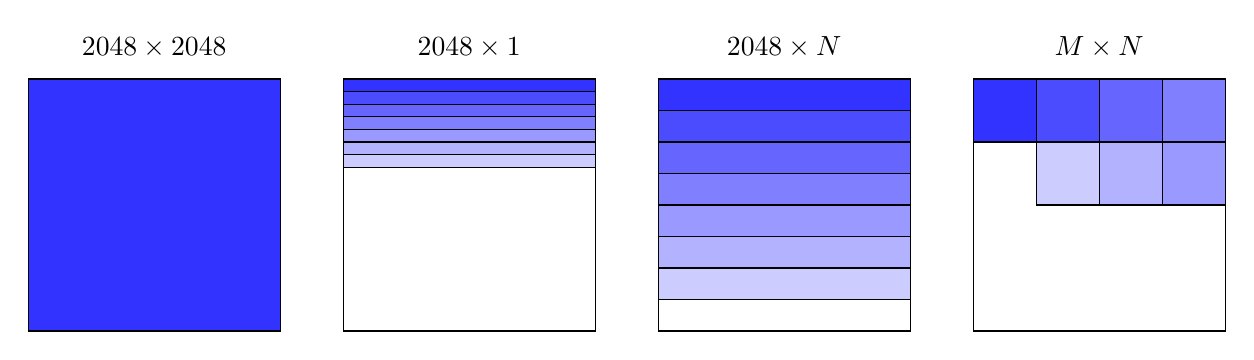
\begin{tikzpicture}[scale=.8]
\draw  (-3,4) rectangle (1,0);
\draw [fill=blue!80] (-3,4) rectangle (1,3.8);
\draw [fill=blue!70] (-3,3.8) rectangle (1,3.6);
\draw [fill=blue!60] (-3,3.6) rectangle (1,3.4);
\draw [fill=blue!50] (-3,3.4) rectangle (1,3.2);
\draw [fill=blue!40] (-3,3.2) rectangle (1,3);
\draw [fill=blue!30] (-3,3) rectangle (1,2.8);
\draw [fill=blue!20] (-3,2.8) rectangle (1,2.6);


\draw  (2,4) rectangle (6,0);
\draw [fill=blue!80] (2,4) rectangle (6,3.5);
\draw [fill=blue!70] (2,3.5) rectangle (6,3);
\draw [fill=blue!60] (2,3) rectangle (6,2.5);
\draw [fill=blue!50] (2,2.5) rectangle (6,2);
\draw [fill=blue!40] (2,2) rectangle (6,1.5);
\draw [fill=blue!30] (2,1.5) rectangle (6,1);
\draw [fill=blue!20] (2,1) rectangle (6,0.5);


\draw  (7,4) rectangle (11,0);
\draw [fill=blue!80] (7,4) rectangle (8,3);
\draw [fill=blue!70] (8,4) rectangle (9,3);
\draw [fill=blue!60] (9,4) rectangle (10,3);
\draw [fill=blue!50] (10,4) rectangle (11,3);
\draw [fill=blue!40] (10,3) rectangle (11,2);
\draw [fill=blue!30] (9,3) rectangle (10,2);
\draw [fill=blue!20] (8,3) rectangle (9,2);

\node at (-6,4.5) {$2048\times2048$};
\node at (-1,4.5) {$2048\times1$};
\node at (4,4.5) {$2048\times N$};
\node at (9,4.5) {$M\times N$};

\draw [fill=blue!80] (-8,4) rectangle (-4,0);
\end{tikzpicture}
    \caption{Different types of scanning motions}
    \label{tkz:scanning_motions}
\end{figure}


\subsection{Resolution} 
\label{ssec:resolution}
The requirement for the altimetry mode changes based on the height. The target is a resolution of at least $0.1\,\%$. To ensure that this requirement is met, both the largest altitude of $8\,km$, and the smallest altitude of $500\,m$ will be investigated.

The minimum resolution for the largest and shortest altitude are $8\,m$ and $0.5\,m$ respectively. The maximum allowable FWHM can be calculated using \cref{eq:max_FWHM}.
 Using \cref{eq:FWHM_sigma} the maximum standard deviation can be calculated. The calculations are performed

\begin{align}\label{eq:max_FWHM}
FWHM_{max} = \frac{2x}{c}
\end{align}

\begin{table}[H]
\centering
\caption{Required standard deviation to meet the system requirements}
\label{tab:AM_requirements}
\begin{tabular}{|l|rr|}\hline
    \textbf{AM requirements} & short & long \\
    \hline 
    altitude & $500\,m$ & $8\,km$ \\
    resolution & $50\,cm$ & $8\,m$ \\
    FWHM & $3.33\,n s$ & $53.33\,n s$ \\
    $\sigma$ & $1.42\,n s$ & $22.65\,n s$ \\
    \hline 
\end{tabular}
\end{table}








% \subsubsection{standard deviation shortcut}
To calculate the standard deviation of the sum of multiple random variables that are independent and uncorrelated, one can use \cref{eq:variance_weighted_sum}


\begin{align}\label{eq:variance_weighted_sum}
\newcommand{\Var}{\mathrm{Var}}
 	\Var[aX+bY+cZ] = a^2\Var[X]+b^2\Var[Y]+c^2\Var[Z]
\end{align}




Next consider a situation where there are two random variable distributions. The first distribution is $S$, which is a normal distribution with $\mu_s=ToF$, where $ToF \in \{0, 50\mu\}$, and $\sigma_s=100p$. The second distribution is $N$, which is a uniform distribution with $\mu_n=\frac{50\mu}{2}$ and $\sigma_n=\frac{50\mu}{\sqrt{12}}$.

\begin{align}
	\mu_{mean} &= \frac{1}{110}\Big(\sum_{k=1}^{100}\mu_s+\sum_{l=1}^{10}\mu_n\Big)\\
			   &= \frac{100ToF+10*25\mu}{110}\\
			   &= \frac{10}{11}ToF+227.3n
\end{align}


\begin{align}
	\mathrm{Var}_{mean} &= \mathrm{Var}\Big[\frac{1}{110}\Big(\sum_{k=1}^{100}S_k+\sum_{l=1}^{10}N_l\Big)\Big]\\ 
	 &= \frac{1}{110^2}\Big(\sum_{k=1}^{100}\mathrm{Var}[S]+\sum_{l=1}^{10}\mathrm{Var}[N]\Big)\\
	&= \frac{1}{110^2}(100\sigma_s^2+10\sigma_n^2)\\
	&= \frac{10^{-18}+2.0833\cdot10^{-9}}{110^2}\\
	&= 1.7218\cdot10^{-13}\\
	\sigma_{mean} &= \sqrt{\mathrm{Var}_{mean}}\\
				  &= 414.94n
\end{align}



% Now we grab 100 samples out of $S$ and 10 out of $N$. First, the $\sigma$ and $\mu$ of the average of the 100 samples of $S$ is calculated.

% \begin{align}
% 	\mu_{s,mean} &= \frac{1}{100}\sum_{k=1}^{100}\mu_s\\
% 			     &= ToF
% \end{align}

% \begin{align}
% 	\mathrm{Var}[\frac{1}{100}\sum_{k=1}^{100}S_k] &= \frac{1}{100^2}\sum_{k=1}^{100} \mathrm{Var}[S_k]\\
% 						  &= \frac{\mathrm{Var}[S]}{100}\\
% 	\sigma_{s,mean} &= \frac{\sigma_s}{\sqrt{100}}\\
% 					&= 10p
% \end{align}

% Next the average of 10 samples of $N$ is calculated.

% \begin{align}
% 	\mu_{n,mean} &= \frac{1}{10}\sum_{k=1}^{10}\mu_n\\
% 			     &= 25\mu
% \end{align}

% \begin{align}
% 	\mathrm{Var}[\frac{1}{10}\sum_{k=1}^{10}] &= \frac{1}{10^2}\sum_{k=1}^{10} \mathrm{Var}[N_k]\\
% 						  &= \frac{\mathrm{Var}[N]}{10}\\
% 	\sigma_{s,mean} &= \frac{\sigma_n}{\sqrt{10}}\\
% 					&= \frac{50\mu}{\sqrt{120}}
% 					&\approx 4.5644\mu
% \end{align}

% Next the two resulting functions are combined


%\subsection{Trade-offs and Methodology} 
\label{ssec:trade_offs_and_methodology}
This section will list the trade-offs that can be found in the system. Each trade-off will be analyzed, and based on that, a decision will be made.


\subsubsection{High Frequency vs Low Frequency pulses}\label{sssec:high_low_freq}
The pulse frequency is limited by the roundtrip time  of the transmitted photons. The roundtrip time can be calculated using \cref{eq:roundtrip}

\begin{align}\label{eq:roundtrip}
t_{round} = \frac{2r}{c}
\end{align}
where $c\approx 3\cdot10^8$ is the speed of light, and $r$ the altitude of the sensor. The maximum pulse frequency can then be calculated using \cref{eq:pulse_f}

\begin{align}\label{eq:pulse_f}
f_{pulse} = \frac{1}{t_{round}} = \frac{c}{2r}
\end{align}

The maximum altitude are different for the Altimetry and Hazard Detection mode. The maximum pulse frequency of both modes is shown in \cref{tab:pulse_frequency}.

\begin{table}[H]
\centering
\caption{Pulse frequency for both modes}
\label{tab:pulse_frequency}
\begin{tabular}{|l|ll|}
\hline
\textbf{Pulse Frequency}      &      Altimetry & Hazard Detection    \\ \hline
Maximum altitude  &  $8\,km$ & $500\, m$\\ 
Roundtrip time      &  $53.3\,\mu s$ & $3.33\,\mu s$ \\
Pulse frequency     & $18.75\,kHz$    & $300\,kHz$  \\ \hline
\end{tabular}
\end{table}


In order to increase the frequency, it is intersting to see what happens if the frequency is increased. The TDC measures the time between the last outgoing pulse and the incomming pulse. This means that the performed measurement $t_{TDC}$ can be calculated using \cref{eq:t_TDC_ToF}.

\begin{align}\label{eq:t_TDC_ToF}
	t_{TDC} &=ToF \mod T_{pulse}\\	
	ToF &= t_{TDC}+k\cdot T_{pulse} & k \in \mathbb{N}\label{eq:ToF_t_TDC}
\end{align}

 where $t_{TDC}$ is the measurement of the TDC, $ToF$ the time of flight, and $T_{pulse}$ the time period of the laser pulses. The returned answer is related to $ToF$ as shown in \cref{eq:ToF_t_TDC}. The precision of the measurement is maintained,  but on a larger scale the information is lost. \\
 \\
To solve this problem one can make measurements in two different frequencies. The idea is also applied in TDCs (Name of technique?), where two ring oscillators with different frequencies are used to amplify the range of the TDC. A similar idea can be applied here, but instead of using two oscillators, the time is devided in half, and in the first half the laser sends pulses in frequency $f_1$, and in the second half pulses with frequncy $f_2$. These two different measurements can first be used to determine the large scale ToF, and then the measurements can be combined to get a high accuracy to accompany that.\\
\\
As a proof of concept. This idea is applied to the Altimetry Mode. It is assumed that a difference of $5\,ns$ between $\lambda_1$ and $\lambda_2$ is sufficient. Now using a maximum $ToF$ one can calculate that optimal two frequencies, such that $f1_>f_2$ and $f_2$ as high as possible. 

\begin{align}
 	\frac{50\mu}{5n} &= 10660\\ 
 	\sqrt{\frac{50\mu}{5n}} &\approx 103
 \end{align} 
 Now two coprime numbers in $\mathbb{N}$ around 103 are 103 and 104. The resulting frequencies are
 \begin{align}
 	T_1 &= 103\cdot5n = 515n\\
 	T_2 &= 104\cdot5n = 520n\\
 	f_1 &= \frac{1}{T_1} = 1.9417\,MHz\\
 	f_2 &= \frac{1}{T_1} = 1.9231\,MHz\\
 \end{align}
The pulse frequency increases by a factor 100. A matlab plot of the resulting system is shown in \cref{fig:frequency_hopping}, where the measurement values of the TDC are plotted against the $ToF$.


\begin{figure}[h]
    \centering
    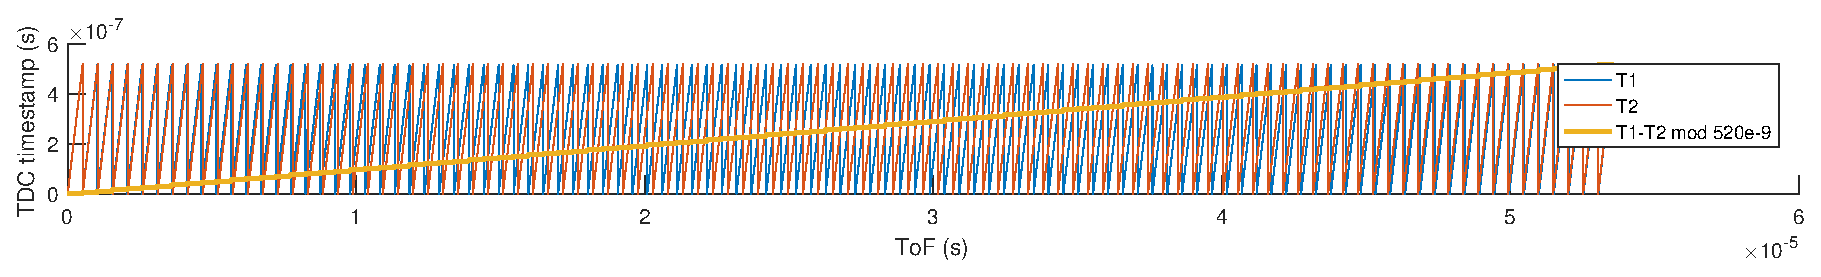
\includegraphics[width=\textwidth]{fig/frequency_hopping.eps}
    \caption{Matlab plot of TDC measurements vs ToF}
    \label{fig:frequency_hopping}
\end{figure}

The $ToF$ can be calculated using \cref{eq:ToF}.

\begin{align}
	t_{1-2} &= (t_1-t_2)\mod T_2\\
	ToF &= \frac{t_{1-2}}{T_2-T_1}T_1+\frac{t_1+t_2-t_{1-2}}{2}\label{eq:ToF}
\end{align}
where $t_1$ and $t_2$ are the timestamp measurements for $f_1$ and $f_2$ respectively. $t_{1-2}$ is the modulus of the time difference between $t_1$ and $t_2$.

\section{Optics}\label{ssec:optics}
The receiver optics are a good place to start of with, because the optics are not very dependent on results achieved in other areas. The optics have to transport as many desired photons, and as little unwanted photons to the active area on the SPADs as possible. All while having an acceptable depth of field. 

The most basic solution is a single lens with an aperture. The opacity of the lens can be calculated with the absorption of the lens material and f-number of the lens using \cref{eq:basic_opacity}.

\begin{align}\label{eq:basic_opacity}
\text{opacity} = \frac{1-\text{absorption}}{\text{f-number}^2}
\end{align}

 The performance of a possible configuration is shown in \cref{tab:basic_optics}

\begin{table}[H]
\centering
\caption{Performance of basic optics solution}
\label{tab:basic_optics}
\begin{tabular}{|l|r|}\hline
    \textbf{Basic Optics} & \\
    \hline 
    f-number & $2.00\, $ \\
    absorption & $5.00\,\%$ \\
    opacity & $23.75\, \%$ \\
    \hline 
\end{tabular}
\end{table}


\subsection{Improvements}
There are a couple of additions that can improve the performance of the optics. The first and essential one, is the use of a bandpass filter. The transmitted signal will have a very specific bandwidth of $850\,nm$. Using a narrow bandpass filter one can filter out an enormous part of the background noise. The filter will have an opacity of $50\,\%$ for the target wavelength.

The captured photons that hit the lens need to be guided to the active area of the SPADs. If the active area on the chip is very small, one can use microlenses to improve the effectiveness of the optics. A Microlens focuses light on a single SPAD on the chip. Two types of microlenses will be considered: a spherical lens, and a square shaped lens. The presence of microlenses poses a limitation of the main lens. The f-number must be relatively large. A higher f-number means a smaller aperture and therefore more loss of photons. A way of dealing with this problem is to use a second lens instead. An overview of the available options is shown in \cref{tkz:receiver_optics}

\begin{figure}[H]
    \centering


\resizebox{\linewidth*3/4}{!}{
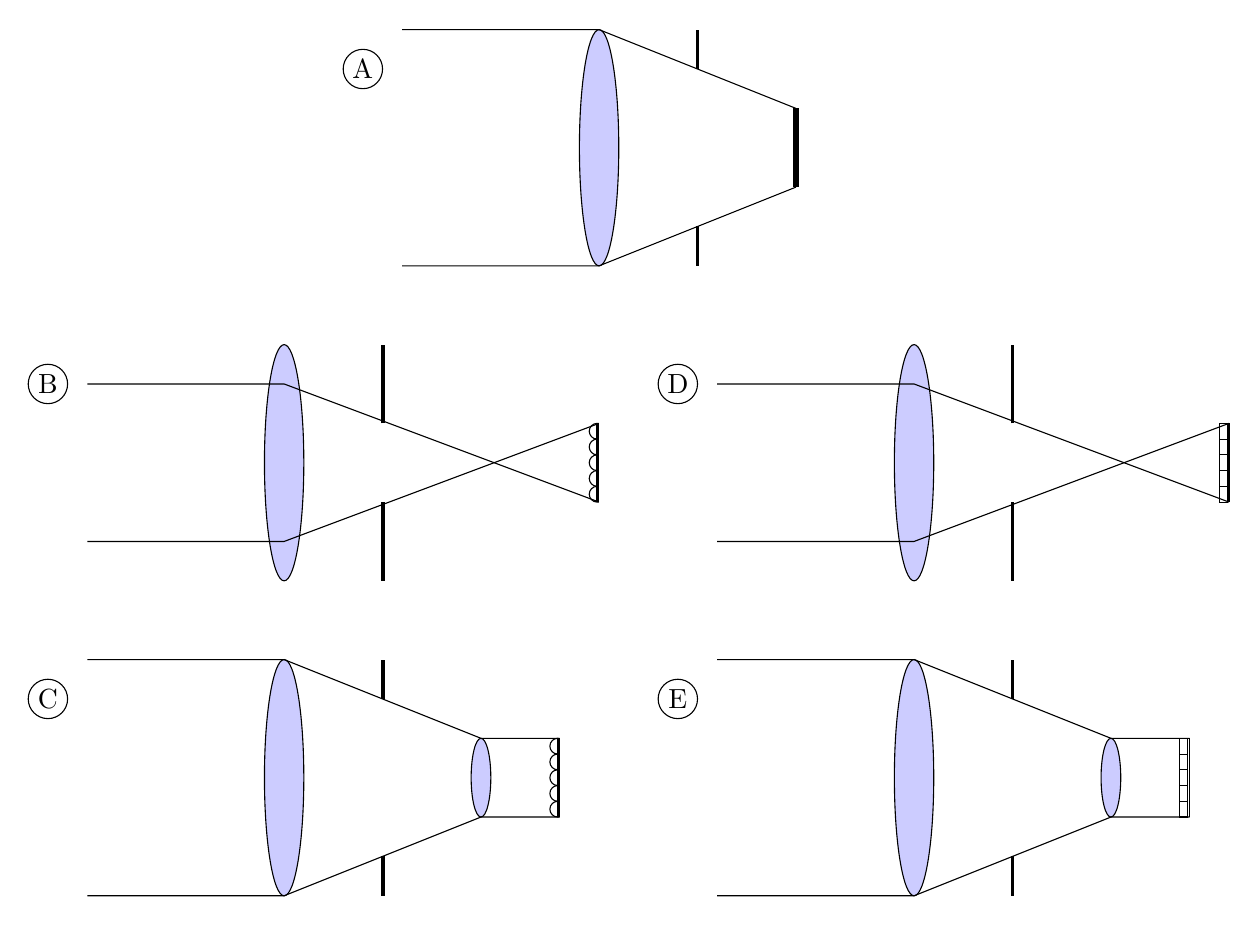
\begin{tikzpicture}[scale=.5]

%%%%%% low F-number, no microlens

%lens
\draw [fill=blue!20] (7,4) ellipse (0.5 and 3);

%diafragma
\draw [line width=.5mm] (9.5,6) -- (9.5,7);
\draw [line width=.5mm] (9.5,1) -- (9.5,2);

%sensitive area
\draw [line width=.7mm] (12,3) -- (12,5);

%light beams
\draw (2,7) to (7,7) to (12,5);
\draw (2,1) to (7,1) to (12,3);

%%%%%%Microlens + high F-number

%lens
\draw [fill=blue!20] (-1,-4) ellipse (0.5 and 3);

%diafragma
\draw [line width=.5mm] (1.5,-3) -- (1.5,-1);
\draw [line width=.5mm] (1.5,-7) -- (1.5,-5);

%sensitive area
\draw [line width=.7mm] (7,-5) -- (7,-3);

%light beams
\draw (-6,-2) to (-1,-2) to (7,-5);
\draw (-6,-6) to (-1,-6) to (7,-3) node (v1) {};


%Microlenses
\draw  (6.95,-3.2) ellipse (.2 and .2);
\draw  (6.95,-3.6) ellipse (.2 and .2);
\draw  (6.95,-4.0) ellipse (.2 and .2);
\draw  (6.95,-4.4) ellipse (.2 and .2);
\draw  (6.95,-4.8) ellipse (.2 and .2);
\fill  (7,-2.8) rectangle (7.4,-5.2) [fill=white];

%%%%%%Microlens + extra lens

%lens
\draw [fill=blue!20] (-1,-12) ellipse (0.5 and 3);

%second lens
\draw [fill=blue!20] (4,-12) ellipse (0.25 and 1);

%diafragma
\draw [line width=.5mm] (1.5,-10) -- (1.5,-9);
\draw [line width=.5mm] (1.5,-15) -- (1.5,-14);

%sensitive area
\draw [line width=.75mm] (6,-13) -- (6,-11);

%light beams
\draw (-6,-9) to (-1,-9) to (4,-11) to (6,-11);
\draw (-6,-15) to (-1,-15) to (4,-13) to (6,-13);


%Microlenses
\draw  (5.95,-11.2) ellipse (.2 and .2);
\draw  (5.95,-11.6) ellipse (.2 and .2);
\draw  (5.95,-12) ellipse (.2 and .2);
\draw  (5.95,-12.4) ellipse (.2 and .2);
\draw  (5.95,-12.8) ellipse (.2 and .2);
\fill  (6,-10.8) rectangle (6.4,-13.2) [fill=white];

%%%%%% Square Microlens + high F-number

%lens
\draw [fill=blue!20] (15,-4) ellipse (0.5 and 3);

%diafragma
\draw [line width=.5mm] (17.5,-3) -- (17.5,-1);
\draw [line width=.5mm] (17.5,-7) -- (17.5,-5);

%sensitive area
\draw  (23,-5) -- (23,-3);

%light beams
\draw (10,-2) to (15,-2) to (23,-5);
\draw (10,-6) to (15,-6) to (23,-3);


%Microlenses
\draw  (22.75,-3) rectangle (22.95,-3.4);
\draw  (22.75,-3.4) rectangle (22.95,-3.8);
\draw  (22.75,-3.8) rectangle (22.95,-4.2);
\draw  (22.75,-4.2) rectangle (22.95,-4.6);
\draw  (22.75,-4.6) rectangle (22.95,-5);


%%%%%% Square Microlens + extra lens

%lens
\draw [fill=blue!20] (15,-12) ellipse (0.5 and 3);

%second lens
\draw [fill=blue!20] (20,-12) ellipse (0.25 and 1);

%diafragma
\draw [line width=.5mm] (17.5,-10) -- (17.5,-9);
\draw [line width=.5mm] (17.5,-15) -- (17.5,-14);

%sensitive area
\draw  (22,-13) -- (22,-11);

%light beams
\draw (10,-9) to (15,-9) to (20,-11) to (22,-11);
\draw (10,-15) to (15,-15) to (20,-13) to (22,-13);


%Microlenses
\draw  (21.75,-11) rectangle (21.95,-11.4);
\draw  (21.75,-11.4) rectangle (21.95,-11.8);
\draw  (21.75,-11.8) rectangle (21.95,-12.2);
\draw  (21.75,-12.2) rectangle (21.95,-12.6);
\draw  (21.75,-12.6) rectangle (21.95,-13);



\draw  (1,6) ellipse (.5 and .5) node[]{A};
\draw  (-7,-2) ellipse (.5 and .5) node[]{B};
\draw  (-7,-10) ellipse (.5 and .5) node[]{C};
\draw  (9,-2) ellipse (.5 and .5) node[]{D};
\draw  (9,-10) ellipse (.5 and .5) node[]{E};


\end{tikzpicture}
}

    \caption{Overview of possible receiver optics implementations}
    \label{tkz:receiver_optics}
\end{figure}

\begin{align}
\text{opacity} = (1-\text{absorption}_1)(1-\text{absorption}_2)\cdot\text{opacity filter}\cdot \frac{X}{\text{f-number}^2}
\end{align}
Where $X$ is the active area on the chip. A comparison between the different options is shown in \cref{tab:receiver_optics}

\begin{table}[H]
\centering
\caption{comparison of different optics solutions}
\label{tab:receiver_optics}
\begin{tabular}{|l|lllll|}\hline
\textbf{Type}                & \textbf{A}        & \textbf{B}        & \textbf{C}        & \textbf{D}        & \textbf{E}        \\ \hline
absorption $1^{st}$ lens & 0.05     & 0.05     & 0.05     & 0.05     & 0.05     \\
f-number                 & 2        & 8        & 2        & 8        & 2        \\
absorption $2^{nd}$ lens & 0        & 0        & 0.05     & 0        & 0.05     \\
active area on chip      & 0.05     & 0.55     & 0.55     & 0.65     & 0.65     \\ \hline
effective opacity            & 0.011875 & 0.008164 & 0.124094 & 0.009648 & 0.146656 \\ \hline
\end{tabular}
\end{table}

The comparison in \cref{tab:receiver_optics} shows some good alternatives to the basic lens, if there is a need for it due to a small active area on the chip. However, most of the future calculations will focus on the basic model A.


\section{Scanning motion}\label{ssec:scanning_motion}
In \cref{ssec:SPADs}, it was concluded that a SPAD array with one SPAD per pixel is not feasible. Therefore a scanning motion is required. Possible scanning motions for different SPAD array configurations are shown in \cref{tkz:scanning_motions}. Note that the $2048\times1$ motion is in essence a special case of the $2048\times N$ motion, where exactly one row of pixels is observed at a time. The $M\times N$, with $M<2048$ and $N<2048$ needs a scanning motion in both $x$ and $y$ direction. This makes the scanning motion very complicated and unreliable. Therefore only the family of solutions with $2048\times N$ with $N<2048$ will be considered.


\begin{figure}[H]
    \centering
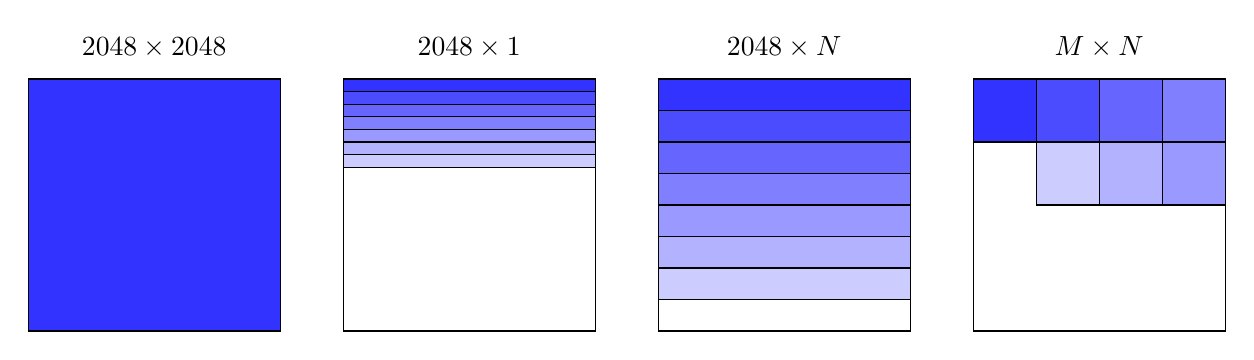
\begin{tikzpicture}[scale=.8]
\draw  (-3,4) rectangle (1,0);
\draw [fill=blue!80] (-3,4) rectangle (1,3.8);
\draw [fill=blue!70] (-3,3.8) rectangle (1,3.6);
\draw [fill=blue!60] (-3,3.6) rectangle (1,3.4);
\draw [fill=blue!50] (-3,3.4) rectangle (1,3.2);
\draw [fill=blue!40] (-3,3.2) rectangle (1,3);
\draw [fill=blue!30] (-3,3) rectangle (1,2.8);
\draw [fill=blue!20] (-3,2.8) rectangle (1,2.6);


\draw  (2,4) rectangle (6,0);
\draw [fill=blue!80] (2,4) rectangle (6,3.5);
\draw [fill=blue!70] (2,3.5) rectangle (6,3);
\draw [fill=blue!60] (2,3) rectangle (6,2.5);
\draw [fill=blue!50] (2,2.5) rectangle (6,2);
\draw [fill=blue!40] (2,2) rectangle (6,1.5);
\draw [fill=blue!30] (2,1.5) rectangle (6,1);
\draw [fill=blue!20] (2,1) rectangle (6,0.5);


\draw  (7,4) rectangle (11,0);
\draw [fill=blue!80] (7,4) rectangle (8,3);
\draw [fill=blue!70] (8,4) rectangle (9,3);
\draw [fill=blue!60] (9,4) rectangle (10,3);
\draw [fill=blue!50] (10,4) rectangle (11,3);
\draw [fill=blue!40] (10,3) rectangle (11,2);
\draw [fill=blue!30] (9,3) rectangle (10,2);
\draw [fill=blue!20] (8,3) rectangle (9,2);

\node at (-6,4.5) {$2048\times2048$};
\node at (-1,4.5) {$2048\times1$};
\node at (4,4.5) {$2048\times N$};
\node at (9,4.5) {$M\times N$};

\draw [fill=blue!80] (-8,4) rectangle (-4,0);
\end{tikzpicture}
    \caption{Different types of scanning motions}
    \label{tkz:scanning_motions}
\end{figure}


\subsubsection{Background Noise}\label{ssec:background_noise}
For the background noise, it is assumed that the sun is the dominant source. The sum is modelled as an ideal black body. The spectral irradiance of the sun can be calculated using \cref{eq:spectral_irradiance}.
\begin{align}\label{eq:spectral_irradiance}
I_\lambda(\lambda,T) = \frac{2hc^2}{\lambda^5}\frac{1}{e^{\frac{hc}{\lambda kT}}-1}
\end{align}
where $I_\lambda(v,t)$ is spectral irradiance with unit $W/m^3$. \\
$h$ is the planck constant\\
$c$ is the speed of light in vacuum \\
$k$ is the Boltzman constant \\
$\lambda$ is the wavelength of the electromagnetic radiation\\
$T$ is the absolute temperature of the body\\
The spectral irradiance of the sun is calculated in \cref{tab:sun_irradiance}.

\begin{table}[H]
\centering
\caption{Calculation of sun irradiation}
\label{tab:sun_irradiance}
\begin{tabular}{|l|ll|} \hline
\textbf{Sun irradiation} &          &                          \\ \hline
$h                        $&$ 6.63\cdot10^{-34} $&$ J\cdot s                 $\\
$c                        $&$ 3.00\cdot10^8     $&$ m/s                      $\\
$k                        $&$ 1.38\cdot10^{-23} $&$ j/K                      $\\
$\lambda                  $&$ 850               $&$ nm                         $\\
$T                        $&$ 5780              $&$ K                        $\\
$I_\lambda                $&$ 1.51\cdot10^{13}  $&$ W/m^3 $\\ \hline
\end{tabular}
\end{table}

The next step is to calculate the power emitted by the sun in the specified bandwidth, at the location of Europa. This is done by modelling sun as a point source, and then spreading that power over a sphere with a radius equal to the distance between the sun and Europa, as is done in \cref{eq:point_source}.

\begin{align}\label{eq:point_source}
    P_{sun} = I_{\text{sun}} B_\lambda S \frac{r_{\text{sun}}^2}{r_{\text{europa}}^2}
\end{align}
where $I_{\text{sun}}$ is the spectral irradiance of the sun at the center frequency of the filter, $B_\lambda$ is the bandwidth of the filter in meters, $S$ the surface area of the target area on Europa, $r_{\text{sun}}$ the of radius of the sun, and $r_{\text{europa}}$ the distance between Europa and the sun. The effective radiance of the background noise at Europa is calculated in \cref{tab:power_background} using \cref{eq:point_source}.

\begin{table}[H]
\centering
\caption{Effective power that hits the target area on Europa}
\label{tab:power_background}
\begin{tabular}{|l|ll|} \hline
\textbf{background power} &                     &         \\ \hline
$I_{lambda}$              & $1.51\cdot10^{13}$  & $W/m^3$ \\
$B$                       & $10$                & $nm$    \\
$S$                       & $15625$             & $m^2$   \\
$r_{sun}$                 & $695700$            & $m$     \\
$r_{europa}$              & $8\cdot10^8$        & $m$     \\
$P_B$                     & $0.179$             & $W$     \\ \hline
\end{tabular}
\end{table}
\subsection{Resolution} 
\label{ssec:resolution}
The requirement for the altimetry mode changes based on the height. The target is a resolution of at least $0.1\,\%$. To ensure that this requirement is met, both the largest altitude of $8\,km$, and the smallest altitude of $500\,m$ will be investigated.

The minimum resolution for the largest and shortest altitude are $8\,m$ and $0.5\,m$ respectively. The maximum allowable FWHM can be calculated using \cref{eq:max_FWHM}.
 Using \cref{eq:FWHM_sigma} the maximum standard deviation can be calculated. The calculations are performed

\begin{align}\label{eq:max_FWHM}
FWHM_{max} = \frac{2x}{c}
\end{align}

\begin{table}[H]
\centering
\caption{Required standard deviation to meet the system requirements}
\label{tab:AM_requirements}
\begin{tabular}{|l|rr|}\hline
    \textbf{AM requirements} & short & long \\
    \hline 
    altitude & $500\,m$ & $8\,km$ \\
    resolution & $50\,cm$ & $8\,m$ \\
    FWHM & $3.33\,n s$ & $53.33\,n s$ \\
    $\sigma$ & $1.42\,n s$ & $22.65\,n s$ \\
    \hline 
\end{tabular}
\end{table}








\subsubsection{standard deviation shortcut}
To calculate the standard deviation of the sum of multiple random variables that are independent and uncorrelated, one can use \cref{eq:variance_weighted_sum}


\begin{align}\label{eq:variance_weighted_sum}
\newcommand{\Var}{\mathrm{Var}}
 	\Var[aX+bY+cZ] = a^2\Var[X]+b^2\Var[Y]+c^2\Var[Z]
\end{align}




Next consider a situation where there are two random variable distributions. The first distribution is $S$, which is a normal distribution with $\mu_s=ToF$, where $ToF \in \{0, 50\mu\}$, and $\sigma_s=100p$. The second distribution is $N$, which is a uniform distribution with $\mu_n=\frac{50\mu}{2}$ and $\sigma_n=\frac{50\mu}{\sqrt{12}}$.

\begin{align}
	\mu_{mean} &= \frac{1}{110}\Big(\sum_{k=1}^{100}\mu_s+\sum_{l=1}^{10}\mu_n\Big)\\
			   &= \frac{100ToF+10*25\mu}{110}\\
			   &= \frac{10}{11}ToF+227.3n
\end{align}


\begin{align}
	\mathrm{Var}_{mean} &= \mathrm{Var}\Big[\frac{1}{110}\Big(\sum_{k=1}^{100}S_k+\sum_{l=1}^{10}N_l\Big)\Big]\\ 
	 &= \frac{1}{110^2}\Big(\sum_{k=1}^{100}\mathrm{Var}[S]+\sum_{l=1}^{10}\mathrm{Var}[N]\Big)\\
	&= \frac{1}{110^2}(100\sigma_s^2+10\sigma_n^2)\\
	&= \frac{10^{-18}+2.0833\cdot10^{-9}}{110^2}\\
	&= 1.7218\cdot10^{-13}\\
	\sigma_{mean} &= \sqrt{\mathrm{Var}_{mean}}\\
				  &= 414.94n
\end{align}



% Now we grab 100 samples out of $S$ and 10 out of $N$. First, the $\sigma$ and $\mu$ of the average of the 100 samples of $S$ is calculated.

% \begin{align}
% 	\mu_{s,mean} &= \frac{1}{100}\sum_{k=1}^{100}\mu_s\\
% 			     &= ToF
% \end{align}

% \begin{align}
% 	\mathrm{Var}[\frac{1}{100}\sum_{k=1}^{100}S_k] &= \frac{1}{100^2}\sum_{k=1}^{100} \mathrm{Var}[S_k]\\
% 						  &= \frac{\mathrm{Var}[S]}{100}\\
% 	\sigma_{s,mean} &= \frac{\sigma_s}{\sqrt{100}}\\
% 					&= 10p
% \end{align}

% Next the average of 10 samples of $N$ is calculated.

% \begin{align}
% 	\mu_{n,mean} &= \frac{1}{10}\sum_{k=1}^{10}\mu_n\\
% 			     &= 25\mu
% \end{align}

% \begin{align}
% 	\mathrm{Var}[\frac{1}{10}\sum_{k=1}^{10}] &= \frac{1}{10^2}\sum_{k=1}^{10} \mathrm{Var}[N_k]\\
% 						  &= \frac{\mathrm{Var}[N]}{10}\\
% 	\sigma_{s,mean} &= \frac{\sigma_n}{\sqrt{10}}\\
% 					&= \frac{50\mu}{\sqrt{120}}
% 					&\approx 4.5644\mu
% \end{align}

% Next the two resulting functions are combined






% \subsection{Laser}
The laser is responsible for the photons that are used for the Time of Flight (ToF) measurement. The laser has to ensure that the Signal to Background Noise Ratio (SBNR) is at least 0 dB. The power budget of the entire system is $50\,W$, which is the main bottleneck for the performance of the laser. The wavelength of the laser is $850\,nm$. The $P_B$ is already calculated in \cref{ssec:background_noise}. In order to achieve an SNR of 0 dB, the signal power $P_S$ must therefore at least match the background noise power that hits the surface of Europa. One can calculate the signal power at the optics using \cref{eq:P_S}.

\begin{align}\label{eq:P_S}
	P_S = P_{pulse} \cdot f_{pulse} \cdot R_{\text{Europa}}
\end{align}
where $P_{pulse}$ is the power of a single pulse of the laser, $f_{pulse}$ the frequency at which the pulses are transmitted, $R_{\text{Europa}}$ the reflectivity of Europa, and $r$ the altitude from the sensor to the surface of Europa. The SBNR can then be calculated using \cref{eq:SBNR}.

\begin{align}\label{eq:SBNR}
	SBNR &= \frac{P_S}{P_B}
\end{align}

The power of a single pulse can be calculated by combining \cref{eq:P_S} and \cref{eq:SBNR} into \cref{eq:p_pulse}. This is done in \cref{tab:p_pulse}.

\begin{align}
	P_{pulse} &= \frac{P_B\cdot SBNR}{f_{pulse}\cdot R_{\text{Europa}}}
\end{align}

\begin{table}[H]
\centering
\caption{Power of a laser pulse}
\label{tab:p_pulse}
\begin{tabular}{|l|ll|} \hline
\textbf{power of a laser pulse}  &              &      \\ \hline
$R_Europa$                       & $0.35        $&      \\
$P_B      $                      & $0.413       $&$ W/m^2 $\\
ground area coverage             & $15625       $&$ m^2   $\\
$SNBR      $                     & $0           $&$ dB   $\\
$f_{pulse}    $                    & $18750       $&$ Hz   $\\
$P_{pulse}     $                   & $0.3441 $&$ W    $\\ \hline
\end{tabular}
\end{table}

The $P_{pulse}$ is the optical power that is emitted by the laser. The electrical power is $\frac{P_{pulse}}{0.1}=3.4\,W$, which is well within the power envelope of $50\,W$. The next step is to calculate the required peak power $p_{peak}$ of the laser, using \cref{eq:p_peak}

\begin{align}\label{eq:p_peak}
 	P_{peak} &= \frac{P_{pulse}}{t_{pulse} \cdot f_{pulse}}
 \end{align} 
where $P_{peak}$ is the peak power and $t_{pulse}$ the FWHM of a pulse.

Using a typical pulse width of $t_{pulse} = 100\,ns$ and the $f_{pulse}$ as calculated in \cref{ssec:high_low_freq} one gets the result shown in \cref{tab:p_peak}.


\begin{table}[H]
\centering
\caption{Peak power calculation}
\label{tab:p_peak}
\begin{tabular}{|l|ll|} \hline
\textbf{Peak laser power} &             &    \\ \hline
$P_{pulse}                 $&$ 0.3441 $&$ W  $\\
$t_{pulse}                  $&$ 1.00\cdot10^{-7}    $&$ s  $\\
$f_{pulse}                  $&$ 18750       $&$ Hz $\\
$P_{peak}                  $&$ 184         $&$ W  $\\ \hline
\end{tabular}
\end{table}















%\clearpage
%\section{Overview} 
\label{sec:overview}

\begin{figure}[H]
    \centering



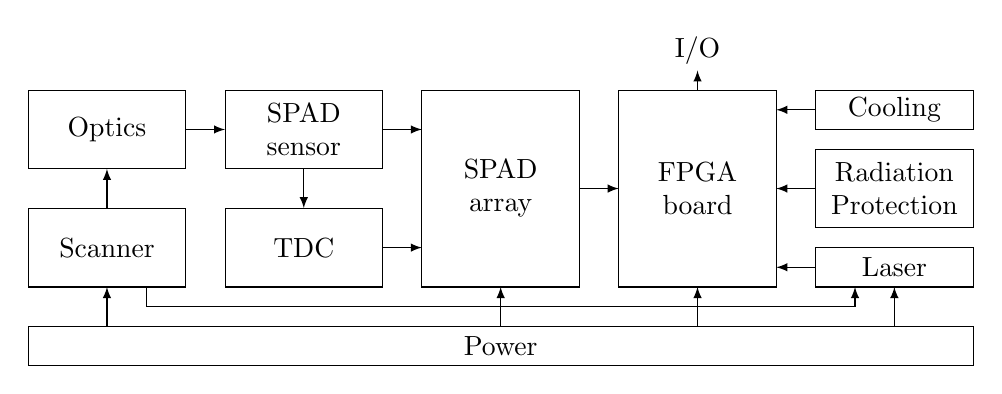
\begin{tikzpicture}[scale=.5]

\draw  (13,2) rectangle (17,1) node[pos=.5, align=center]{Cooling};
\draw  (13,0.5) rectangle (17,-1.5) node[pos=.5, align=center]{Radiation\\Protection};
\draw  (-7,-4) rectangle (17,-5) node[pos=.5, align=center]{Power};
\draw  (13,-2) rectangle (17,-3) node[pos=.5, align=center]{Laser};
\draw  (8,2) rectangle (12,-3) node[pos=.5, align=center]{FPGA\\board};
\draw  (3,2) rectangle (7,-3) node[pos=.5, align=center]{SPAD\\array};
\draw  (-2,2) rectangle (2,0) node[pos=.5, align=center]{SPAD\\sensor};
\draw  (-7,2) rectangle (-3,0) node[pos=.5, align=center]{Optics};
\draw  (-7,-1) rectangle (-3,-3) node[pos=.5, align=center]{Scanner};
\draw  (-2,-1) rectangle (2,-3) node[pos=.5, align=center]{TDC};

\draw [>=latex, ->](0,0) -- (0,-1);
\draw [>=latex, ->](2,-2) -- (3,-2);
\draw [>=latex, ->](13,1.5) -- (12,1.5);
\draw [>=latex, ->](7,-.5) -- (8,-.5);
\draw [>=latex, ->](2,1) -- (3,1);
\draw [>=latex, ->](13,-2.5) -- (12,-2.5);
\draw [>=latex, ->](10,2) -- (10,2.5);
\draw [>=latex, ->](-3,1) -- (-2,1);
\draw [>=latex, ->](13,-.5) -- (12,-.5);
\draw [>=latex, ->](5,-4) -- (5,-3);
\draw [>=latex, ->](10,-4) -- (10,-3);
\draw [>=latex, ->](15,-4) -- (15,-3);
\draw [>=latex, ->](-5,-1) -- (-5,0);
\node at (10,3) {I/O};

\draw [>=latex, ->](-5,-4) -- (-5,-3);
\draw [>=latex, ->](-4,-3) -- (-4,-3.5) -- (14,-3.5) -- (14,-3);

\end{tikzpicture}




    \caption{Schematic overview}
    \label{tkz:schematic_overview}
\end{figure}

\section{SPAD sensor} 
\label{sec:spad_sensor}
The SPAD Sensor generates a pulse when a photon is detected. It is connected to a TDC, and is used to construct a SPAD grid.

\subsection{requirements} 
\label{ssec:sensor_req}

\begin{table}[H]
    \begin{tabular}{l|l|l}
    ~                                  & Threshold & Goal \\ \hline
    Max Acquisition Slant Range        & 5 km      & 8 km \\
    Min Operational Range              & 5 m       & 1 m  \\
    Range Accuracy                     & 10 cm     & 5 cm \\
    Photon Detection Probability (PDP) & ?         & ?    \\
    Dead-time                          & ?         & ?    \\
    Dark count rate (DCR)              & ?         & ?    \\
    \end{tabular}
\end{table}

The most important requirement of the SPAD is the range accuracy of 5-10 cm. 

\begin{align*}
	\frac{5\cdot10^-2}{3\cdot10^8} &= 167\, ps 
\end{align*}

Therefore the jitter on the time between the arrival of a photon and the transmission of a pulse must be as small as possible.

\subsection{Possibilities} 
\label{ssec:sensor_pos}
To be continued

\subsection{Choice} 
\label{ssec:sensor_choice}
Basically we are going for CMOS Si SPAD's.


\section{TDC} 
\label{sec:tdc}
The Time intrerval to Digital Converted (TDC) is connected to a (or several) SPAD sensor. The TDC has to convert the difference in time between two pulses into a digital representation. It is used together with the SPAS sensors to build a SPAD grid.

\subsection{Requirements} 
\label{ssec:tdc_req}

\begin{table}[H]
    \begin{tabular}{l|l|l}
    ~                    & Threshold & Goal   \\ \hline
    accuracy             & 50 ps?    & 30 ps? \\
    jitter               & 30 ps?    & 10 ps? \\
    area per SPAD sensor & ?         & ?      \\
    power usage          & ?         & ?      \\
    \end{tabular}
\end{table}

\subsection{Possibilities} 
\label{ssec:tdc_pos}
There are a lot of possibilities here. But I don't know what technique they use to save on the amount of TDC's.

\subsection{Choice} 
\label{ssec:tdc_choice}


\section{SPAD grid} 
\label{sec:spad_grid}
The grid is the structure that implements the SPAD sensors and TDC's into a grid to measure 

\subsection{Requirements} 
\label{ssec:grid_req}

\begin{table}[H]
    \begin{tabular}{l|l|l}
    ~                                    & Threshold         & Goal              \\ \hline
    Update rate                          & 0.1 Hz            & 1 Hz              \\
    Ground Sample Distance               & 10 cm             & 5 cm              \\
    Ground Area Coverage at max altitude & 100 m times 100 m & 125 m times 125 m \\
    Time for 3D map creation             & 1 s               & 1 s               \\
    \end{tabular}
\end{table}

\subsection{Possibilities} 
\label{ssec:grid_pos}

\subsection{Choice} 
\label{ssec:grid_choice}
The unproposed master thesis board.

\section{FPGA board} 
\label{sec:fpga_board}

\subsection{Requirements} 
\label{ssec:grid_req}

\begin{table}[H]
    \begin{tabular}{l|l|l}
    ~                                    & Threshold         & Goal              \\ \hline
    Update rate                          & 0.1 Hz            & 1 Hz              \\
    Ground Sample Distance               & 10 cm             & 5 cm              \\
    Ground Area Coverage at max altitude & 100 m times 100 m & 125 m times 125 m \\
    Time for 3D map creation             & 1 s               & 1 s               \\
    \end{tabular}
\end{table}

Note that the relevant requirements are similar to the SPAD grid, because the SPAD grid has to generate the data, and the FPGA has to process it. 

\subsection{Possibilities} 
\label{ssec:grid_pos}

\subsection{Choice} 
\label{ssec:grid_choice}
The FPGA accompanying the unproposed master thesis board.

\section{Radiation protection} 
\label{sec:radiation_protection}

Because we cannot change the FPGA board to be more resilient against radiation. It  ight be necessary to protect the board with external components. 
\subsection{Requirements} 
\label{ssec:grid_req}

The FPGA has to survive a certain amounty of Cobalt-64 and proton radiation.

\subsection{Possibilities} 
\label{ssec:grid_pos}
The possibilities vary between different kinds of materials, different thickness, and positions. The possibility of no protection is also present.\\
\\


\subsection{Choice} 
\label{ssec:grid_choice}
The unproposed master thesis board.

\section{Laser} 
\label{sec:laser}



\end{document}




















